\documentclass[a4paper,12pt]{ltxdoc}
\usepackage[utf8]{inputenc}
\usepackage[T1]{fontenc}
\usepackage{a4wide}
\usepackage{graphicx}\graphicspath{{./figs/}}
\usepackage{wrapfig}\setlength{\intextsep}{0ex}
\usepackage{rotating}

\usepackage{soccerbars}

% -- ETH and team colors
\definecolor{ethblue}{RGB}{31,64,122}
\definecolor{ethred}{RGB}{168,50,45}
\definecolor{reds}{HTML}{C8102E}
\definecolor{skyblues}{RGB}{108,171,221} % 6CABDD
\definecolor{nerazzurri}{HTML}{0267AB}
\definecolor{fcbayern}{HTML}{DC052D}
\definecolor{bayernblau}{HTML}{0066B2}
\definecolor{schwarzgelb}{HTML}{FDE100}
\definecolor{schalke}{RGB}{0,75,156} % 004D9D

\usepackage[pdftex,colorlinks,
    urlcolor=ethred,linkcolor=ethred,citecolor=ethblue,%
    pdftitle={The soccerbars Package},%
    pdfsubject={Word-sized tallies for series of association football match results},%
    pdfauthor={Ulrik Brandes}
   ]{hyperref}

% -----------------------------------------------------------------
\title{The \textsf{soccerbars} Package for \LaTeX\thanks{%
Soccerbars are based on
previous work with Bobo Nick (while at the University of Konstanz),
discussions with David Schoch (The University of Manchester),
and prototyping with Lukas Knoflach (TU~Graz).
Eren Akbiyik (ETH Z\"urich) provides implementations of soccerbars
for use with python and~R at \url{https://github.com/snlab-eakbiyik/soccerbars}.}\\
\normalsize ---~version 0.7~---}
\author{Ulrik Brandes, ETH Zürich}
\date{2021-03-14}
% -----------------------------------------------------------------

\begin{document}
% =================================================================
\maketitle
% -----------------------------------------------------------------
\begin{abstract}
The \textsf{soccerbars} package provides macros
to generate word-sized tallies
for series of association football (soccer) match results. 
They are meant to enrich league tables and the discussion of streaks
with the actual sequences of results.
\end{abstract}
% -----------------------------------------------------------------
\tableofcontents
\clearpage

\section{Introduction}
% =================================================================

Since the very first season of the Football League in 1888/1889, 
and the introduction of the 2-point system a few matchdays in,
news reports feature league tables 
recording the number of matches played,
wins, losses, draws, accumulated goals for and against, and points.
These data have later been augmented with goal differences,
and are sometimes broken down into results home and away.

Another, more detailed, representation
that compactly records all results of an entire season,
albeit not in the order in which they came about,
are cross-tables.
The following combination of detailed and summarized information
was printed as part of a season wrap-up in
\emph{The Cricket and Football Field},
a weekly sports paper out of Bolton~\cite{fl1889}.%
\footnote{The one result missing is an Everton loss at West Bromwich
which is, however, printed in the home team's row.}
 
% -----------------------------------------------------------------
\begin{flushright}
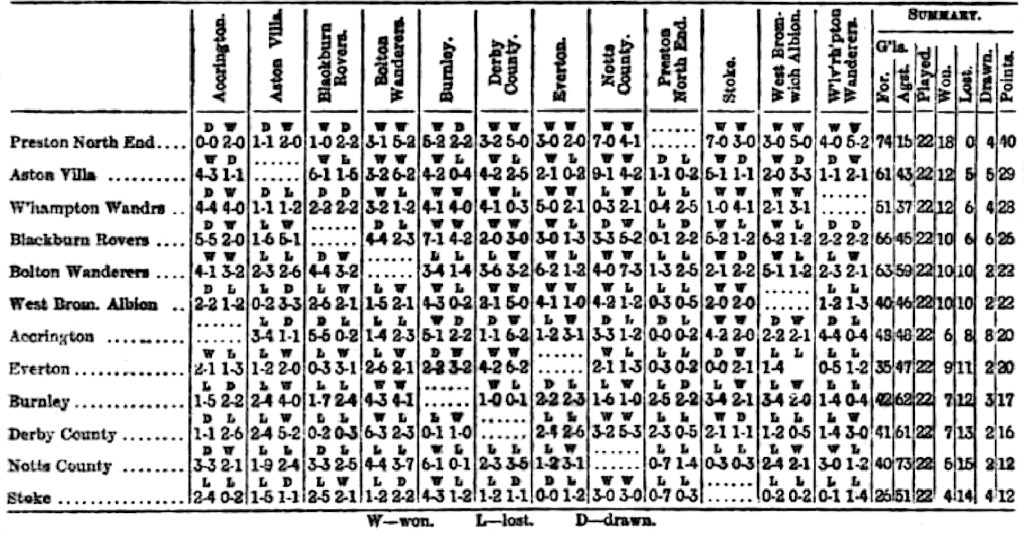
\includegraphics[width=\linewidth]{fl1889_cff}
\scriptsize\quad\color{gray}\begin{tabular}{r@{}}
Newspaper image \copyright~The British Library Board. All rights reserved.\\
With thanks to The British Newspaper Archive (\url{www.britishnewspaperarchive.co.uk})
\end{tabular}
\end{flushright}
% -----------------------------------------------------------------

A perspective that is supported by neither representation, 
but the subject of many a conversation, are series:
going unbeaten in 34~matches,
conceding only two goals in the first eleven matches with a new manager,
losing six in a row at home, and so on. 
Despite frequently referring to a team's form, or recent performance,
the closest news reports come to non-verbal representations of such series 
are charts depicting a team's wins, draws, and losses
over the last maybe five, seven, or ten matches.

This is what soccerbars are made for: compact representations
designed to integrate a sequence of results into text, tables, and graphics.
Below is the first season of the Football League
showing for each team all of its results
in the order in which the matches were played. 

\begin{center}
\sf\sbZeroDots
\renewcommand{\arraystretch}{1.2}
\begin{tabular}{rlcrrrrrr}\hline
\textbf{\#} 
   & \textbf{Team} & \textbf{Season}
   & \textbf{W} & \textbf{D} & \textbf{L}
   & ~\textbf{GF} & \textbf{GA} & \textbf{Pts}\\\hline
 1 & Preston North End & 
   \soccerbar{(5-2),(0-4)*,(3-1),(2-3)*,(7-0),(3-0),(0-0)*,(5-2),(0-7)*,(1-1),(0-3)*}\,%
   \soccerbar{(2-0),(2-5)*,(5-0),(2-2)*,(3-0),(0-5)*,(1-0),(4-1),(2-2)*,(0-2)*,(0-2)*}
   & 18 & 4 &  0 & 74 & 15 & 40 \\
 2 & Aston Villa &
   \soccerbar{(1-1)*,(5-1),(2-1),(9-1),(2-0)*,(6-1),(2-3)*,(4-3),(1-1)*,(1-1)*,(5-1)*}\,%
   \soccerbar{(2-1),(2-4)*,(1-1)*,(4-2),(4-2),(4-0)*,(6-2),(2-0),(3-3)*,(0-2),(5-2)*}
   & 12 & 5 &  5 & 61 & 43 & 29 \\
 3 & Wolverhampton Wanderers &
   \soccerbar{(1-1),(0-4),(4-1),(2-2),(4-4)*,(0-4)*,(2-2)*,(5-2)*,(4-1),(3-2),(0-1)*}\,%
   \soccerbar{(2-1)*,(4-0),(2-1),(4-1),(2-1)*,(1-3)*,(3-0)*,(3-0)*,(4-0),(1-2)*,(2-1)}
   & 12 & 4 &  6 & 51 & 37 & 28 \\
 4 & Blackburn Rovers &
   \soccerbar{(5-5),(6-2),(2-2)*,(3-3)*,(6-1)*,(2-2),(5-2),(1-7)*,(3-0),(5-1),(0-2)*}\,%
   \soccerbar{(2-1)*,(4-4),(5-2),(2-1)*,(1-0)*,(2-2),(0-2)*,(3-2)*,(4-2),(3-1)*,(3-0)}
   & 10 & 6 &  6 & 66 & 45 & 26 \\
 5 & Bolton Wanderers &
   \soccerbar{(3-6),(3-4),(3-1)*,(6-2),(4-1)*,(2-1),(2-3),(2-1)*,(1-5)*,(3-2)*,(1-2)}\,%
   \soccerbar{(2-5),(4-4)*,(4-1),(2-3)*,(2-1),(6-2)*,(2-2)*,(3-2),(0-4)*,(7-3),(2-3)*}
   & 10 & 2 & 10 & 63 & 59 & 22 \\
 6 & West Bromwich Albion &
   \soccerbar{(0-2)*,(1-2)*,(6-2)*,(4-3),(5-0),(3-0)*,(4-2),(2-2),(1-5),(2-0)*,(1-2)*}\,%
   \soccerbar{(2-1)*,(1-4)*,(2-1)*,(2-1),(0-5),(2-0),(1-3),(2-1)*,(2-0)*,(3-3),(1-0)}
   & 10 & 2 & 10 & 40 & 46 & 22 \\
 7 & Accrington &
   \soccerbar{(2-1)*,(5-5)*,(1-1)*,(2-4)*,(4-4),(6-2),(0-0),(4-3)*,(2-2)*,(3-3)*,(2-0)*}\,%
   \soccerbar{(2-1),(5-1),(4-0)*,(1-1),(4-1)*,(3-1),(2-2)*,(0-2),(1-2),(2-3),(2-0)}
   &  6 & 8 &  8 & 48 & 48 & 20 \\
 8 & Everton &
   \soccerbar{(2-1),(2-1),(2-1)*,(6-2)*,(2-0),(3-1)*,(2-4)*,(6-2),(2-1),(3-0)*,(2-2)*}\,%
   \soccerbar{(3-2),(1-4),(0-0)*,(3-0)*,(3-1)*,(2-1),(0-2),(4-0)*,(1-2),(1-0)*,(3-1)}
   &  9 & 2 & 11 & 35 & 47 & 20 \\
 9 & Burnley &
   \soccerbar{(5-2)*,(3-4)*,(4-1)*,(4-3)*,(4-1),(0-4),(4-3)*,(6-1)*,(1-7),(2-0),(2-2)}\,%
   \soccerbar{(3-2)*,(5-1)*,(2-1),(2-2),(4-2)*,(1-0),(4-0),(2-2),(1-0),(4-2)*,(1-0)*}
   &  7 & 3 & 12 & 42 & 62 & 17 \\
10 & Derby County &
   \soccerbar{(3-6)*,(1-2),(1-1),(2-3),(5-0)*,(6-2)*,(2-4),(6-2)*,(4-1)*,(0-2),(5-0)*}\,%
   \soccerbar{(3-2),(2-3),(4-2)*,(3-0),(1-0)*,(2-1),(1-0),(5-2),(3-5)*,(1-1)*,(3-0)*}
   &  7 & 2 & 13 & 41 & 61 & 16 \\
11 & Notts County &
   \soccerbar{(2-1)*,(3-0)*,(9-1)*,(3-3),(3-1),(4-2)*,(6-1),(0-7),(3-3),(0-3),(2-4)}\,%
   \soccerbar{(5-2)*,(3-2)*,(1-0)*,(4-1)*,(2-1),(3-0),(1-2)*,(2-1)*,(0-4),(7-3)*,(3-5)}
   &  5 & 2 & 15 & 40 & 73 & 12 \\
12 & Stoke &
   \soccerbar{(0-2),(5-1)*,(3-0),(2-4),(7-0)*,(2-1)*,(4-3),(5-2)*,(1-1),(0-3),(0-1)}\,%
   \soccerbar{(0-3)*,(2-1),(2-1)*,(0-0),(4-1)*,(2-0)*,(2-1)*,(2-2),(2-1)*,(1-1),(2-0)*}
   &  4 & 4 & 14 & 26 & 51 & 12 \\\hline
\end{tabular}
\end{center}

Each tally represents one match result, and it is gray for away matches.
Wins are depicted as forward leaning, draws vertical, and losses backward leaning.
The length above and below the horizontal baseline represent goals for and against. 
It is readily observed that only two out of 132~matches ended in a goalless draw
(Preston N.E.\ at Accrington and Everton at Stoke),
and that winners Preston North End had by far the most clean sheets
(13, marked with small dots where a single-goal line would end).
Other than the loss-less season of the first winners, 
the improvement of Bolton and Derby during the second round is notable,
whereas the opposite can be said of Everton.
Like Everton, teams in the bottom half of the table 
each tallied only a single away win all season;
except Derby County who actually had two, and rather wild ones.

Fast forward 131~years, Liverpool had a stunning season
{\sbZeroDots\begin{soccerbarenv}
\home{4}{1} \away{1}{2} \home{3}{1} \away{0}{3}
\home{3}{1} \away{1}{2} \away{0}{1} \home{2}{1}
\away[reds]{1}{1} \home{2}{1} \away{1}{2} \home{3}{1}
\away{1}{2} \home{2}{1} \home{5}{2} \away{0}{3}
\home{2}{0} \away{0}{2} \away{0}{4} \home{1}{0}
\home{2}{0} \away{0}{1} \home{2}{0} \away{1}{2}
\home{4}{0} \away{0}{1} \home{3}{2} \away[reds]{3}{0}
\home{2}{1} \away[reds]{0}{0} \home{4}{0}
\end{soccerbarenv}\,\soccerbar{(4-0)*,(2-0),(1-3)*,(1-1),(2-1)*,(5-3),(1-3)*}}
as well,
with only {\color{reds}two draws} and {\color{reds}one loss}
(none of them at home)
in the 31~matches they needed to claim the 2019/2020 Premiership.

With a waiting time of {\color{schalke}29~matches} in between
{\sbZeroDots\begin{soccerbarenv}[schalke]
\home[black]{2}{0} \away{5}{0} \away{0}{0} \home{1}{1}
\away{0}{0} \home{0}{5} \away{3}{0} \home{1}{1}
\away{4}{0} \home{0}{3} \away{2}{1} \home{0}{1}
\away{1}{1} \home{1}{1} \away{2}{1} \home{1}{4}
\away{4}{0}
\end{soccerbarenv}\,%
\begin{soccerbarenv}[schalke]
\away{8}{0} \home{1}{3} \away{4}{0} \home{1}{1}
\away{3}{0} \home{1}{1} \away{2}{2} \home{0}{2}
\away{4}{1} \home{0}{3} \away{2}{2} \home{0}{2}
\home{0}{1} \away{3}{0} \home[black]{4}{0} \away[black]{3}{1} \home[black]{1}{2}
\end{soccerbarenv}}
two wins across the second half of the 2019/2020 season and first half of 2020/2021,
Schalke just barely avoided to match the longest non-winning streak
{\sbZeroDots\begin{soccerbarenv}[schalke]
\home[black]{2}{0} \away{5}{0} \home{0}{2} \away{5}{1}
\home{0}{2} \away{7}{2} \home{1}{5} \away{0}{0}
\home{0}{2} \away{3}{0} \home{0}{6} \away{5}{0}
\home{0}{5} \away{4}{0} \away{3}{1} \home{1}{2}
\home{0}{2}
\end{soccerbarenv}\,%
\begin{soccerbarenv}[schalke]
\away{3}{0} \home{0}{0} \away{3}{1} \home{0}{4}
\away{2}{1} \home{0}{1} \away{5}{0} \home{1}{1}
\away{2}{0} \home{0}{9} \away{4}{0} \home{1}{1}
\away{4}{0} \home{0}{3} \away{3}{1} \home[black]{2}{1} \away[black]{4}{0}
\end{soccerbarenv}}
in Bundesliga history, a record set by Tasmania Berlin
in their single season of membership
in the top flight, 1965/1966.


\section{Design}\label{sec:design}
% =================================================================

Soccerbars are micro-visualizations
that integrate with text
to support and illustrate statements with detailed data.

They instantiate Edward Tufte's marvelous idea of sparklines~\cite{tufte},
i.e., to use intense, word-sized, high-resolution graphics
to present extensive sequence data within eyespan.
Sparklines are popular for univariate time-series data such as stock prices,
and available in the \textsf{sparklines} package~\cite{sparklines}.

Since soccer results are multivariate
(goals for and against, points awarded, home or away), 
there are different ways of encoding them in sparklines
and, indeed, a number of alternatives have been proposed.
Some of them straightforward, others rather involved.

Soccerbars have been derived from a design principle
systematically extending the concept of sparklines. 
Instead of combining sparklines for multiple attributes,
gestaltlines~\cite{gestaltlines,gestaltmatrix} align glyphs
designed to exploit Gestalt theory 
and thus facilitate the perception of
trends, shifts, and outliers in multivariate sequences.


\subsection{Basics}
% -----------------------------------------------------------------

The primary metaphor is that of a tally.
Instead of keeping separate tallies for wins, losses, and draws 
the result categories are distinguished by slant. 
A winning team can be thought of as charging forward
and a losing team as skidding.

\begin{wrapfigure}{r}{6em}
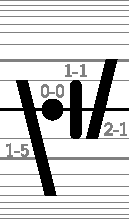
\includegraphics[width=\linewidth]{basics}
\end{wrapfigure}
The slant is fixed rather than, say,
dependent on the goal difference,
to visually group stretches of results in the same category. 

To represent goals for and against, the length of tallies is varied. 
Horizontal clipping at a goal-dependent height
is preferred over goal-dependent lengths, though,
because it yields an alignment of the number of goals a team scored
no matter the outcome (and thus slant). 

This idea is reinforced visually by clipping tallies for wins and losses horizontally. 
Caps of vertical tallies for draws are rounded
to emphasize the difference from the other two outcomes,
and place them more clearly in the same category as the dots for goalless matches. 

In the majority of matches, no side scores more than two goals,
but on occasion a team may well rack up eight or even more. 
The height at which a tally is clipped is therefore increased
roughly according to the frequency with which the next goal occurs,
and capped at nine. 
This limits the height required and favors the more frequent cases
at the expense of differences in the regime where they matter less.


\subsection{Extensions}
% -----------------------------------------------------------------

The basic design can be augmented with two kinds of annotations 
that reference features of common interest explicitly.

% -----------------------------------------------------------------
\begin{wrapfigure}{r}{8em}
\definecolor{bleu}{HTML}{0055A4}
\definecolor{rouge}{HTML}{EF4135}
\newcommand\france{%
\begin{soccerbarenv}[bleu]
\score{2}{1} \score{1}{0} \score{0}{0}
\score[rouge]{4}{3} \score[rouge]{2}{0} \score[rouge]{1}{0} \score[rouge]{4}{2}
\end{soccerbarenv}}
% -----------------------------------------------------------------
\huge\hfill%
\begin{tabular}{c@{~}c@{}}
\france               & \sbZeroDots\france\\
\sbTwoGoalLine\france & \sbZeroDots\sbTwoGoalLine\france
\end{tabular}
\end{wrapfigure}
% -----------------------------------------------------------------
France's road to victory at the World Cup Finals 2018 is shown four times on the right.
The group phase of three matches is followed by four elimination rounds.
Extra dots at the level of a single goal (top right soccerbar)
facilitate counting the number of matches
in which a team or its opponents did not score,
and their alignment simultaneously creates the visual effect of another horizontal line
because of the frequency of such events.

To distinguish better between higher scores,
in spite of the non-linear scaling of heights,
an extra line can be added at the statistically important threshold of two goals (bottom left). 
This can be seen, for instance,
for the~\mbox{4--3} against Argentina in the round of the last sixteen
and the~\mbox{4--2} against Croatia in the final. 

Both extensions can be added independently via package options
and switched on and off in the document as described in Section~\ref{sec:options}.  


\subsection{Alignment with Text}
% -----------------------------------------------------------------

When displayed within text, soccerbars are vertically centered
such that the levels of one goal for and against
correspond to the height of the character `x' and the baseline,
i.e., they are |1ex| apart.
High scores are allowed to stick out and overlap other content,
as the \LaTeX\ bounding box
deliberately extends only to the levels of two goals for and against
to avoid affecting the distance between baselines in a paragraph.

Over the last five and a half seasons, El Cl\'asico,
restricted to matches in La Liga,
looked as follows 
\begin{quote}

\includegraphics[width=\linewidth]{clasico}
\end{quote}
from either perspective.

While line thickness, slant, and horizontal spacing can be altered
as described in Section~\ref{sec:settings},
vertical spacing is tied to the size of the current font
via length unit~|ex|.



\section{Using the Package}
% =================================================================
\newcommand\lfcfirstround{(4-1),(1-2)*,(3-1),(0-3)*,(3-1),(1-2)*,(0-1)*,(2-1),(1-1)*,(2-1),(1-2)*,(3-1),(1-2)*,(2-1),(5-2),(0-3)*,(2-0),(0-2)*,(0-4)*}
\newcommand\lfcsecondround{(1-0),(2-0),(0-1)*,(2-0),(1-2)*,(4-0),(0-1)*,(3-2),(3-0)*,(2-1),(0-0)*,(4-0),(4-0)*,(2-0),(1-3)*,(1-1),(2-1)*,(5-3),(1-3)*}
\newcommand\lfcseason{\lfcfirstround,\lfcsecondround}

The \textsf{soccerbars} package
provides three different ways
to include word-size tallies of soccer results
into \LaTeX\ documents: a macro, an environment, and a file reader. 
They all produce the same kind of visualization 
but differ in the intended usage scenario.


\subsection{Loading and Options}\label{sec:options}
% -----------------------------------------------------------------

To make use of \textsf{soccerbars},
the file |soccerbars.sty| should be
obtained from \url{https://github.com/ubrandes-ethz/soccerbars}
and placed in a directory
searched by the \LaTeX\ installation.
It is loaded by placing
\begin{quote}
  \cs{usepackage}\oarg{options}\marg{soccerbars}
\end{quote}
in the preamble of a \LaTeX\ document. 
Several other packages will be loaded automatically,
because \textsf{soccerbars} depends explicitly on
Ti\emph{k}Z~\cite{tikz}, \textsf{csvsimple}~\cite{csvsimple}, and \textsf{etoolbox}~\cite{etoolbox},
each with their own dependencies.

The following three package options allow to toggle design variants
introduced in Section~\ref{sec:design} and the distinction of away matches.
\begin{description}
\item[\tt zerodots] Marks each time that a team did not score a goal with a little dot tangential to the imaginary line at one goal. This makes it easier to appreciate that Liverpool went only three times without a goal {\sbZeroDots\soccerbar{\lfcseason}} but had fifteen clean sheets, and even eight in a row. 
\item[\tt twogoalline] Adds an extra horizontal lines to mark the two-goal level with half the width of the zero-goal baseline. Thus, higher scores are more easily distinguished. Liverpool lost the two away matches out of those three in which they conceded more than two goals {\sbTwoGoalLine\soccerbar{\lfcseason}} but won all fourteen matches in which they scored more than two goals. 
\item[\tt outlined] With this option, away matches are marked by outlining rather than a change in brightness. While the difference may be hard to tell \soccerbar{\lfcfirstround}\,{\sbOutlined\soccerbar{\lfcsecondround}} in small font, it creates an aesthetic of its own in large displays such as
\raisebox{-1ex}{\Large\sbOutlined\soccerbar{\lfcseason}}~.

\end{description}
Three options can be combined arbitrarily. Declaring, for instance,
\begin{quote}
  \cs{usepackage[zerodots,twogoalline]\{soccerbars\}}
\end{quote}
yields soccerbars such as {\sbZeroDots\sbTwoGoalLine\soccerbar{\lfcseason}}\,.
Initially, only those design choices declared in package options are active,
but in the document all three can be switched on and off using commands
\begin{quote}\begin{tabular}[b]{lll}
\cs{sbZeroDots} & \cs{sbTwoGoalLine} & \cs{sbOutlined} \\
\cs{sbNoZeroDots} & \cs{sbNoTwoGoalLine} & \cs{sbNotOutlined}
\end{tabular}.\end{quote}
These commands apply locally within the current group,
i.e., switching on no-goal dots temporarily by |{\sbZeroDots ...}|
does not require switching off.

The change of colors and more basic stylistic adjustments
are described in Sections~\ref{sec:colors} and~\ref{sec:settings}.


\subsection{Generating Soccerbars}\label{sec:macros}
% -----------------------------------------------------------------

Macro, environment, file reader

\begin{description}
\item[\cs{soccerbar}\marg{results}]
  This macro is the most straightforward way to generate a soccerbar.
  Its argument is a comma-separated list of match results
  in the form |(|\meta{goals for}|-|\meta{goals against}|)|
  for matches in which the current team is playing at home
  and |(|\meta{goals against}|-|\meta{goals for}|)*| 
  in which it is playing away.
  As an example, consider this rocky start to a season
  \begin{quote}
  \begin{verbatim}
\soccerbar{(2-2), (0-3)*,(6-1), (1-1)*,(4-0),
           (2-3)*,(1-2), (2-2)*,(2-1), (5-1)*}\end{verbatim}
  \end{quote}
  culminating in a loss at home
  \soccerbar{(2-2),(0-3)*,(6-1),(1-1)*,(4-0),(2-3)*,(1-2),(2-2)*,(2-1),(5-1)*}
  and a thrashing away. 
  While some clubs might content themselves with it,
  a more club one may well sack its manager at this point.
\item[\cs{begin\{soccerbarenv\}} \dots \cs{end\{soccerbarenv\}}]
  With the |soccerbarenv| environment,
  the identical soccerbar as above is obtained in more verbose form as
  \begin{quote}
  \begin{verbatim}
\begin{soccerbarenv}
  \home{2}{2} \away{0}{3} \home{6}{1}
  \away{1}{1} \home{4}{0} \away{2}{3}
  \home{1}{2} \away{2}{2} \home{2}{1}
  \away{5}{1}
\end{soccerbarenv}\end{verbatim}
  \end{quote}
  The motivation for this alternative specification is that both the environment and 
  the \cs{home} and \cs{away} commands have optional parameters
  by which colors can be changed per result, rather than for the entire soccerbar. 
  This is described in more detail in the next section.
 
  Note that, as in real life, \cs{home\{1\}\{2\}} and \cs{away\{2\}\{1\}}
  generally do not look the same,
  because away matches may be rendered differently.
\item[\cs{csvsoccerbar}\marg{team}\marg{first match}\marg{last match}]
  For many, long, or partial sequences,
  it may be more convenient to gather match results from a file. 
  It is assumed that they are stored in CSV (\emph{comma separated values}) format
  with one match per row and four separate columns for
  home and away team names and the numbers of goals they scored.
  The filename and headers are declared once using the command 
  \cs{sbCSVnames}\marg{file}\linebreak[2]%
  \marg{hometeam}\linebreak[2]\marg{awayteam}\linebreak[2]%
  \marg{homegoals}\linebreak[2]\marg{awaygoals}
  and \cs{csvsoccerbar}\marg{team}\linebreak[2]%
  \marg{first match}\linebreak[2]\marg{last match}
  then yields a soccerbar for this team depicting results
  on the specified interval of matchdays
  (assuming they appear in the correct order in the file).
  
  From a file |bl2019-20.csv| tabulating results as 
  \begin{quote}
  \begin{verbatim}
Spieltag,Heim,HT,GT,Gast
1,Bayern,2,2,Hertha BSC
1,Dortmund,5,1,Augsburg
...\end{verbatim}
  \end{quote}
  the above start of the season and its continuation are obtained via
  \begin{quote}
  \begin{verbatim}
\sbCSVnames{bl2019-20.csv}{Heim}{Gast}{HT}{GT}
...
\csvsoccerbar{Bayern}{1}{10}
\csvsoccerbar{Bayern}{11}{34}\end{verbatim}
  \end{quote}
  This yields
  \soccerbar{(2-2),(0-3)*,(6-1),(1-1)*,(4-0),(2-3)*,(1-2),(2-2)*,(2-1),(5-1)*}\,% FCB Kovacz
  \soccerbar{(4-0),(0-4)*,(1-2),(2-1)*,(6-1),(1-3)*,(2-0),(0-4)*,(5-0),(1-3)*,(0-0),(1-4)*,(3-2),(0-6)*,(2-0),(0-2)*,(5-2),(0-1)*,(5-0),(2-4)*,(2-1),(0-1)*,(3-1),(0-4)*} % FCB Flick
  for the season, or one stepping stone to another treble.

  It is important to ensure that
  the encoding of the CSV file is the same as that of the \LaTeX\ document,
  especially if team names contain accents or umlauts.
\end{description}
Scheduled matches that have not been played, yet, can be specified as
|(-)|, |(-)*|, |\home{}{}|, |\away{}{}|, or missing entries in the CSV file
and result in prolonged soccerbars
\soccerbar{(5-1),(1-3)*,(3-1)*,(4-0),(2-2)*,(2-2),(2-2)*,(1-0),(0-0)*,(3-0),(4-0)*,(3-3),(1-2)*,(5-0),(0-4)*,(3-3),(2-1)*}\,\soccerbar{(3-5)*,(5-1),(5-0),(4-3)*,(4-0),(0-2)*,(1-0),(1-2)*,(4-0),(0-2)*,(-),(-),(-),(-),(-),(-),(-)} % BVB until before 0-1 against FCB
with zerodot-sized marks for upcoming matches. 
This is useful in the display of current standings,
when hopes may still run high.

 
\subsection{Changing Colors}\label{sec:colors}
% -----------------------------------------------------------------
\newcommand\cityseason{(0-5)*,(2-2),(1-3)*,(4-0),(3-2)*,(8-0),(1-3)*,(0-2),(0-2)*,(3-0),(2-1),(3-1)*,(2-1),(2-2)*,(1-4)*,(1-2),(0-3)*,(3-1),(3-2)*,(2-0),(2-1),(1-6)*,(2-2),(0-1)*,(2-0)*,(2-0),(0-1)*,(2-0)*,(3-0),(5-0),(2-1)*,(4-0),(1-0)*,(5-0),(0-5)*,(2-1),(0-4)*,(5-0)}
\newcommand\interseason{(4-0),(1-2)*,(1-0),(0-2)*,(1-0),(1-3)*,(1-2),(3-4)*,(2-2),(1-2)*,(1-2)*,(2-1),(0-3)*,(2-1),(0-0),(1-1)*,(4-0),(1-3)*,(1-1),(1-1)*,(1-1),(0-2)*,(4-2),(2-1)*,(2-0)*,(2-1),(3-3),(1-2)*,(6-0),(1-2)*,(2-2)*,(3-1),(0-4)*,(2-2)*,(0-0),(0-3)*,(2-0),(0-2)*}
\newcommand\bvbseason{(5-1),(1-3)*,(3-1)*,(4-0),(2-2)*,(2-2),(2-2)*,(1-0),(0-0)*,(3-0),(4-0)*,(3-3),(1-2)*,(5-0),(0-4)*,(3-3),(2-1)*,(3-5)*,(5-1),(5-0),(4-3)*,(4-0),(0-2)*,(1-0),(1-2)*,(4-0),(0-2)*,(0-1),(1-6)*,(1-0),(0-1)*,(0-2),(0-2)*,(0-4)}

Soccerbars are set in the current foreground color,
by default with somewhat lighter shading of away matches. 
The base color can be set explicitly with an optional parameter
available for both the \cs{soccerbar} macro and the |soccerbarenv| environment.
Whether away matches are lighter, darker, or unaltered
is determined by commands 
\cs{sbAwayBrighter} (default), \cs{sbAwayDarker}, and \cs{sbAwayKeepColor}.
\begin{quote}
  \begin{minipage}[b]{0.75\linewidth}
  \begin{verbatim}
\definecolor{skyblues}{RGB}{108,171,221}
\definecolor{nerazzuri}{HTML}{0267AB}
\definecolor{schwarzgelb}{HTML}{FDE100}
...
\soccerbar[skyblues]{(0-5)*,(2-2),...}
\sbAwayDarker
\soccerbar[nerazzurri]{(4-0),(1-2)*,...}
\soccerbar[schwarzgelb]{(5-1),(1-3)*,...}\end{verbatim}
  \end{minipage}%
  \begin{minipage}[b]{0.25\linewidth}
    \soccerbar[skyblues]{\cityseason}\\[-0.5ex]
    \sbAwayDarker\\[-0.25ex]
    \soccerbar[nerazzurri]{\interseason}\\[-0.25ex]
    \soccerbar[schwarzgelb]{\bvbseason}
  \end{minipage}
\end{quote}
Colors are specified according to the \textsf{xcolor} package~\cite{xcolor}
which is automatically loaded by Ti\emph{k}Z.
Effects \cs{sbAwayBrighter} and \cs{sbAwayDarker} are realized by rendering away matches
in colors |.!66!white| and |.!66!black|, respectively. 

More detailed color choices are possible with the |soccerbarenv| environment. 
To be able to highlight, say, the above mentioned losses {\color{bayernblau}at home} 
\begin{soccerbarenv}
  \home{2}{2} \away{0}{3} \home{6}{1} \away{1}{1} \home{4}{0} \away{2}{3}
  \home[bayernblau]{1}{2}
  \away{2}{2} \home{2}{1}
  \away[fcbayern]{5}{1}
\end{soccerbarenv}
and {\color{fcbayern}away}, an optional color parameter is accepted for each tally.
\begin{quote}
  \begin{verbatim}
\begin{soccerbarenv}
  \home{2}{2} \away{0}{3} \home{6}{1} \away{1}{1} \home{4}{0} \away{2}{3}
  \home[blue]{1}{2} \away{2}{2} \home{2}{1} \away[red]{5}{1}
\end{soccerbarenv}\end{verbatim}
\end{quote}
Changing colors according betting odds
shows that not only the club had higher expectations.
In the following, 
the predicted probability of winning encoded in betting odds 
is used to determine a tally's color on a gradient from white to red:
the more red the less expected the outcome.
\begin{quote}
  \begin{verbatim}
{\sbAwayKeepColor\begin{soccerbarenv}[gray]
  \home[red!85!white]{2}{2} \away[white!74!red]{0}{3}
  \home[white!92!red]{6}{1} \away[red!54!white]{1}{1}
  \home[white!88!red]{4}{0} \away[white!87!red]{2}{3}
  \home[red!89!white]{1}{2} \away[red!85!white]{2}{2}
  \home[white!90!red]{2}{1} \away[red!70!white]{5}{1}
\end{soccerbarenv}}\end{verbatim}
\end{quote}
Half of these
{\sbAwayKeepColor\begin{soccerbarenv}[gray]
  \home[fcbayern!85!white]{2}{2}
  \away[white!74!fcbayern]{0}{3}
  \home[white!92!fcbayern]{6}{1}
  \away[fcbayern!54!white]{1}{1}
  \home[white!88!fcbayern]{4}{0}
  \away[white!87!fcbayern]{2}{3}
  \home[fcbayern!89!white]{1}{2}
  \away[fcbayern!85!white]{2}{2}
  \home[white!90!fcbayern]{2}{1}
  \away[fcbayern!70!white]{5}{1}
\end{soccerbarenv}}
ten matches, and three of the last four, ended rather unexpectedly.

\clearpage
\subsection{Other Settings}\label{sec:settings}
% -----------------------------------------------------------------

Most design choices other than the package options
can be altered with the command
\cs{sbSettings}\linebreak[2]%
\marg{thickness}\linebreak[2]%
\marg{zerodots}\linebreak[2]%
\marg{zeroline}\linebreak[2]%
\marg{slant}\linebreak[2]%
\marg{spacing}\linebreak[2]%
\marg{padding}. 
The six mandatory arguments are described below.
Their default values can be re-established with
\cs{sbDefaults}, which invokes
\begin{quote}
  \cs{sbSettings\{0.18\}\{0.6\}\{0.2\}\{14\}\{0.9\}\{0.2\}} 
\end{quote}
and also \cs{sbAwayBrighter} to set the lighter shading for away matches.
\begin{description}
\item[\meta{thickness}] The thickness of a tally,
  specified as a multiple of |ex|, the height of an `x' in the current font.
  This makes the thickness of tallies scale with their height and spacing.
  Other line widths are relative to this one. 
  The default value of |0.18ex| is based on the stroke width of common fonts.
  Dots for a goalless draw have a matching radius,
  and are thus twice as wide as a tally.
\item[\meta{zerodots}] The diameter of the disk indicating that a team did not score,
  specified as a multiple of the first parameter. 
  For these to be visible, option |zerodots| must have been included
  when loading the package or activated with \cs{sbZeroDots}.
\item[\meta{zeroline}] The thickness of the horizontal line at zero goals,
  specified as a multiple of the first parameter.
  Lines at the level of two goals are drawn at half the thickness, if any.
\item[\meta{slant}] The slant of a tally signifying a win or loss,
  i.e., the angle by which it is rotated out of the vertical position,
  specified in degrees.
  The default value of~|14| is based on the slant of common fonts.
  \begin{center}
    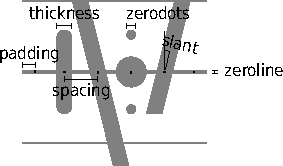
\includegraphics[width=0.4\linewidth]{settings}
  \end{center}
\item[\meta{spacing}] Space between the centers of consecutive tallies on the zero line,
  specified in multiples of the one-goal level (which, in turn, is fixed at |0.5ex|).
  The default of~|0.9| thus corresponds to equidistant placement of tallies every |0.45ex|.
  With the default thickness of |0.18ex|,
  the |0.27ex| gaps between equally slanted tallies
  are wider than the line width, avoiding irritating patterns,
  and dots for consecutive goalless scores do not touch. 
\item[\meta{padding}] The length by which the horizontal line at zero goals
  is extended to the left and right,
  specified in multiples of the one-goal level (which, in turn, is fixed at |0.5ex|).
  The default value of~|0.2| is generally sufficient
  to prevent slanted tallies from sticking out.
\end{description}


\section{The 2019/2020 Season}
% =================================================================

Across Europe, the 2019/2020~season was suspended in March~2020
and, except for France, resumed in May or June.
The following tables therefore show soccerbars
divided into three segments corresponding to the first round,
the second round until the break due to the pandemic,
and the rest of the season.
In the Swiss Super League, teams play each other four times.

\sbZeroDots
\renewcommand{\arraystretch}{1.2}
% -----------------------------------------------------------------

\subsection{Premier League}
% -----------------------------------------------------------------

{\sf\begin{tabular}{@{}rlcrrrr@{~}rrr} \hline
\textbf{\#} 
   & \textbf{Club} & \textbf{Season}
   & \textbf{W} & \textbf{D} & \textbf{L}
   & \textbf{GF} & \textbf{GA} & \textbf{GD}
   & \textbf{P} \\ \hline 
 1 & Liverpool & 
   \soccerbar{(4-1),(1-2)*,(3-1),(0-3)*,(3-1),(1-2)*,(0-1)*,(2-1),(1-1)*,(2-1),(1-2)*,(3-1),(1-2)*,(2-1),(5-2),(0-3)*,(2-0),(0-2)*,(0-4)*}\,%
   \soccerbar{(1-0),(2-0),(0-1)*,(2-0),(1-2)*,(4-0),(0-1)*,(3-2),(3-0)*,(2-1)}\,%
   \soccerbar{(0-0)*,(4-0),(4-0)*,(2-0),(1-3)*,(1-1),(2-1)*,(5-3),(1-3)*}
   & 32 & 3 & 3 & 85 & 33 & 52 & 99 \\
 2 & Manchester City & 
   \soccerbar{(0-5)*,(2-2),(1-3)*,(4-0),(3-2)*,(8-0),(1-3)*,(0-2),(0-2)*,(3-0),(2-1),(3-1)*,(2-1),(2-2)*,(1-4)*,(1-2),(0-3)*,(3-1),(3-2)*}\,%
   \soccerbar{(2-0),(2-1),(1-6)*,(2-2),(0-1)*,(2-0)*,(2-0),(0-1)*,(2-0)*}\,%
   \soccerbar{(3-0),(5-0),(2-1)*,(4-0),(1-0)*,(5-0),(0-5)*,(2-1),(0-4)*,(5-0)}
   & 26 & 3 & 9 & 102 & 35 & 67 & 81 \\
 3 & Manchester United & 
   \soccerbar{(4-0),(1-1)*,(1-2),(1-1)*,(1-0),(2-0)*,(1-1),(1-0)*,(1-1),(1-3)*,(1-0)*,(3-1),(3-3)*,(2-2),(2-1),(1-2)*,(1-1),(2-0)*,(4-1)}\,%
   \soccerbar{(0-2)*,(2-0)*,(4-0),(2-0)*,(0-2),(0-0),(0-2)*,(3-0),(1-1)*,(2-0)}\,%
   \soccerbar{(1-1)*,(3-0),(0-3)*,(5-2),(0-3)*,(2-2),(0-2)*,(1-1),(0-2)*}
   & 18 & 12 & 8 & 66 & 36 & 30 & 66 \\
 4 & Chelsea & 
   \soccerbar{(4-0)*,(1-1),(2-3)*,(2-2),(2-5)*,(1-2),(2-0),(1-4)*,(1-0),(2-4)*,(1-2)*,(2-0),(2-1)*,(0-1),(2-1),(3-1)*,(0-1),(0-2)*,(0-2)}\,%
   \soccerbar{(1-2)*,(1-1)*,(3-0),(2-0)*,(2-2),(2-2)*,(0-2),(2-1),(2-2),(4-0)}\,%
   \soccerbar{(1-2)*,(2-1),(3-2)*,(3-0),(2-3)*,(3-0)*,(1-0),(5-3)*,(2-0)}
   & 20 & 6 & 12 & 59 & 54 & 15 & 66 \\ \hline
 5 & Leicester City & 
   \soccerbar{(0-0),(1-1)*,(1-2)*,(3-1),(1-0)*,(2-1),(5-0),(2-1)*,(2-1),(0-9)*,(0-2)*,(2-0),(0-2)*,(2-1),(2-0),(1-4)*,(1-1),(3-1)*,(0-4)}\,%
   \soccerbar{(1-2)*,(0-3)*,(1-2),(2-1)*,(4-1),(2-2),(0-0)*,(0-1),(1-0)*,(4-0)}\,%
   \soccerbar{(1-1)*,(0-0),(2-1)*,(3-0),(1-1)*,(4-1)*,(2-0),(3-0)*,(0-2)}
   & 18 & 8 & 12 & 67 & 41 & 26 & 62 \\
 6 & Tottenham Hotspur & 
   \soccerbar{(3-1),(2-2)*,(0-1),(2-2)*,(4-0),(2-1)*,(2-1),(3-0)*,(1-1),(2-1)*,(1-1)*,(1-1),(2-3)*,(3-2),(2-1)*,(5-0),(1-2)*,(0-2),(2-1)}\,%
   \soccerbar{(2-2)*,(1-0)*,(0-1),(0-0)*,(2-1),(2-0),(2-3)*,(2-1)*,(2-3),(1-1)*}\,%
   \soccerbar{(1-1),(2-0),(3-1)*,(1-0),(0-0)*,(2-1),(1-3)*,(3-0),(1-1)*}
   & 16 & 11 & 11 & 61 & 47 & 14 & 59 \\ \hline
 7 & Wolverhampton Wanderers & 
   \soccerbar{(0-0)*,(1-1),(1-1),(3-2)*,(2-5),(1-1)*,(2-0),(0-2)*,(1-1),(1-1)*,(1-1)*,(2-1),(1-2)*,(1-1),(2-0),(2-2)*,(1-2),(1-2)*,(3-2)}\,%
   \soccerbar{(1-0)*,(2-1)*,(1-1),(2-3)*,(1-2),(0-0)*,(0-0),(3-0),(2-3)*,(0-0)}\,%
   \soccerbar{(0-2)*,(1-0),(0-1)*,(0-2),(1-0)*,(3-0),(1-1)*,(2-0),(2-0)*}
   & 15 & 14 & 9 & 51 & 40 & 11 & 59 \\
 8 & Arsenal & 
   \soccerbar{(0-1)*,(2-1),(3-1)*,(2-2),(2-2)*,(3-2),(1-1)*,(1-0),(1-0)*,(2-2),(1-1),(2-0)*,(2-2),(2-2)*,(1-2),(1-3)*,(0-3),(0-0)*,(1-1)*}\,%
   \soccerbar{(1-2),(2-0),(1-1)*,(1-1),(2-2)*,(0-0)*,(4-0),(3-2),(1-0)}\,%
   \soccerbar{(3-0)*,(2-1)*,(0-2)*,(4-0),(0-2)*,(1-1),(2-1)*,(2-1),(1-0)*,(3-2)}
   & 14 & 14 & 10 & 56 & 48 & 8 & 56 \\ 
 9 & Sheffield United & 
   \soccerbar{(1-1)*,(1-0),(1-2),(2-2)*,(0-1),(0-2)*,(0-1),(0-0)*,(1-0),(1-1)*,(3-0),(1-1)*,(3-3),(1-1)*,(0-2),(1-2)*,(2-0),(0-1)*,(1-1)}\,%
   \soccerbar{(2-0)*,(2-0)*,(1-0),(1-1)*,(0-1),(0-1)*,(2-1),(1-1),(1-0)}\,%
   \soccerbar{(0-0)*,(3-0)*,(3-0)*,(3-1),(1-1)*,(1-0),(3-0),(2-0)*,(0-1),(3-1)*}
   & 14 & 12 & 12 & 39 & 39 & 0 & 54\\ 
10 & Burnley & 
   \soccerbar{(3-0),(2-1)*,(1-1)*,(0-3),(1-1)*,(2-0),(2-0)*,(1-0),(2-1)*,(2-4),(3-0)*,(3-0),(0-3)*,(0-2),(1-4),(5-0)*,(1-0),(0-1)*,(1-0)*}\,%
   \soccerbar{(0-2),(1-2),(3-0)*,(2-1),(0-2)*,(0-0),(1-2)*,(3-0),(0-0)*,(1-1)}\,%
   \soccerbar{(5-0)*,(1-0),(0-1)*,(1-1),(0-1)*,(1-1)*,(1-1),(0-2)*,(1-2)}
   & 15 & 9 & 14 & 43 & 50 & -7 & 54 \\
11 & Southampton & 
   \soccerbar{(3-0)*,(1-2),(0-2)*,(1-1),(0-1)*,(1-3),(2-1)*,(1-4),(1-1)*,(0-9),(2-1)*,(1-2),(2-2)*,(2-1),(2-1),(2-1)*,(0-1),(1-3)*,(0-2)*}\,%
   \soccerbar{(1-1),(1-0),(1-2)*,(2-3),(0-2)*,(4-0)*,(1-2),(2-0),(3-1)*,(0-1)}\,%
   \soccerbar{(0-3)*,(0-2),(1-3)*,(1-0),(1-1)*,(2-2)*,(1-1),(0-2)*,(3-1)}
   & 15 & 7 & 16 & 51 & 60 & -9 & 52 \\
12 & Everton & 
   \soccerbar{(0-0)*,(1-0),(2-0)*,(3-2),(3-1)*,(0-2),(1-3),(1-0)*,(2-0),(3-2)*,(1-1),(1-2)*,(0-2),(2-1)*,(5-2)*,(3-1),(1-1)*,(0-0),(1-0)}\,%
   \soccerbar{(1-2)*,(2-1)*,(1-0),(1-1)*,(2-2),(2-3)*,(3-1),(3-2)*,(1-1),(4-0)*}\,%
   \soccerbar{(0-0),(0-1)*,(2-1),(1-0)*,(1-1),(3-0)*,(1-1),(0-1)*,(1-3)}
   & 13 & 10 & 15 & 44 & 56 & -12 & 49 \\
13 & Newcastle United & 
   \soccerbar{(0-1),(3-1)*,(0-1)*,(1-1),(3-1)*,(0-0),(5-0)*,(1-0),(1-0)*,(1-1),(2-3)*,(2-1),(2-0)*,(2-2),(0-2)*,(2-1),(1-0)*,(1-0),(4-1)*}\,%
   \soccerbar{(1-2),(0-3),(1-1)*,(1-0),(2-2)*,(0-0),(4-0)*,(1-0)*,(0-0),(0-1)*}\,%
   \soccerbar{(3-0),(1-1),(1-4)*,(2-2),(5-0)*,(2-1)*,(1-3),(0-0)*,(1-3)}
   & 11 & 11 & 16 & 38 & 58 & -20 & 44 \\
14 & Crystal Palace & 
   \soccerbar{(0-0),(1-0)*,(1-2)*,(1-0),(4-0)*,(1-1),(2-0),(1-2)*,(0-2),(2-2)*,(0-2),(2-0)*,(1-2),(0-2)*,(1-0),(0-0)*,(1-1),(1-0)*,(2-1)}\,%
   \soccerbar{(1-1)*,(1-1)*,(1-1),(2-2)*,(0-2),(0-1),(3-1)*,(1-0),(0-1)*,(1-0)}\,%
   \soccerbar{(0-2)*,(4-0)*,(0-1),(3-0)*,(2-3),(2-0)*,(0-2),(2-0)*,(1-1)}
   & 11 & 10 & 17 & 31 & 50 & -19 & 43 \\
15 & Brighton and Hove Albion & 
   \soccerbar{(0-3)*,(1-1),(0-2),(4-0)*,(1-1),(0-0)*,(2-0)*,(3-0),(2-1)*,(3-2),(2-0),(3-1)*,(0-2),(2-1)*,(1-2)*,(2-2),(1-1)*,(0-1),(2-1)*}\,%
   \soccerbar{(2-0),(1-1),(1-0)*,(1-1),(3-1)*,(3-3)*,(1-1),(1-1)*,(0-1),(0-0)*}\,%
   \soccerbar{(2-1),(0-0)*,(0-3),(0-1)*,(1-3),(0-5),(1-1)*,(0-0),(1-2)*}
   & 9 & 14 & 15 & 39 & 54 & -15 & 41 \\
16 & West Ham United & 
   \soccerbar{(0-5),(1-1)*,(1-3)*,(2-0),(0-0)*,(2-0),(2-2)*,(1-2),(2-0)*,(1-1),(2-3),(3-0)*,(2-3),(0-1)*,(2-0)*,(1-3),(0-1)*,(2-1)*,(1-2)}\,%
   \soccerbar{(4-0),(1-0)*,(1-1),(4-1)*,(0-2),(3-3),(2-0)*,(3-2)*,(3-1),(1-0)*}\,%
   \soccerbar{(0-2),(2-0)*,(3-2),(2-2)*,(0-1),(0-4)*,(3-1),(1-1)*,(1-1)}
   & 10 & 9 & 19 & 49 & 62 & -13 & 39 \\ 
17 & Aston Villa & 
   \soccerbar{(3-1)*,(1-2),(2-0),(1-0)*,(0-0),(3-2)*,(2-2),(1-5)*,(2-1),(3-0),(1-2),(2-1)*,(2-0),(2-2)*,(2-1)*,(1-4),(2-0)*,(1-3),(1-0)}\,%
   \soccerbar{(3-0)*,(1-2)*,(1-6),(1-1)*,(2-1),(2-1)*,(2-3),(2-0)*,(4-0)*}\,%
   \soccerbar{(0-0),(1-2),(1-1)*,(0-1),(2-0)*,(0-3),(2-0),(1-1)*,(1-0),(1-1)*}
   & 9 & 8 & 21 & 41 & 67 & -26 & 35 \\ \hline
18 & Bournemouth & 
   \soccerbar{(1-1),(1-2)*,(1-3),(3-1)*,(3-1),(1-3)*,(2-2),(1-0)*,(0-0),(0-0)*,(1-0),(2-1)*,(1-2),(3-2)*,(1-0)*,(0-3),(0-1)*,(0-1),(1-1)}\,%
   \soccerbar{(2-0)*,(4-0)*,(0-3),(1-0)*,(3-1),(2-1),(2-1)*,(3-0)*,(2-2),(2-1)*}\,%
   \soccerbar{(0-2),(1-0)*,(1-4),(5-2)*,(0-0),(4-1),(2-1)*,(0-2),(1-3)*}
   & 9 & 7 & 22 & 40 & 65 & -25 & 34 \\ 
19 & Watford & 
   \soccerbar{(0-3),(1-0)*,(1-3),(1-1)*,(2-2),(8-0)*,(2-0)*,(0-0),(1-1)*,(0-0),(1-2),(0-2)*,(0-3),(2-1)*,(2-0)*,(0-0),(2-0)*,(2-0),(1-1)*}\,%
   \soccerbar{(3-0),(2-1),(0-3)*,(0-0),(2-1)*,(2-3),(1-1)*,(3-0)*,(3-0),(1-0)*}\,%
   \soccerbar{(1-1),(1-0)*,(2-3),(3-0)*,(2-1),(2-1),(3-1)*,(0-4),(3-2)*}
   & 8 & 10 & 20 & 26 & 64 & -28 & 34 \\ 
20 & Norwich City & 
   \soccerbar{(4-1)*,(3-1),(2-3),(2-0)*,(3-2),(2-0)*,(2-0)*,(1-5),(0-0)*,(1-3),(2-0)*,(0-2),(0-2)*,(2-2),(2-1)*,(1-2),(1-1)*,(1-2),(1-0)*}\,%
   \soccerbar{(2-2),(1-1),(4-0)*,(1-0),(2-1)*,(0-0)*,(0-1),(3-0)*,(1-0),(1-0)*}\,%
   \soccerbar{(0-3),(0-1),(4-0)*,(0-1),(2-1)*,(0-4),(1-0)*,(0-2),(5-0)*}
   & 5 & 6 & 27 & 26 & 75 & -49 & 21 \\\hline
\end{tabular}}


\clearpage
\subsection{La Liga}
% -----------------------------------------------------------------

{\sf\begin{tabular}{rlcrrrr@{~}rrr} \hline 
\textbf{\#}
   & \textbf{Equipo} & \textbf{Resultados}
   & \textbf{PG} & \textbf{PE} & \textbf{PP}
   & \textbf{GF} & \textbf{GC} & \textbf{GD}
   & \textbf{Pts} \\ \hline 
 1 & Real Madrid &
     \soccerbar{(1-3)*,(1-1),(2-2)*,(3-2),(0-1)*,(2-0),(0-0)*,(4-2),(1-0)*,(5-0),(0-0),(0-4)*,(3-1),(1-2)*,(2-0),(1-1)*,(0-0)*,(0-0),(0-3)*}\,%
     \soccerbar{(2-1),(0-1)*,(1-0),(1-4)*,(2-2),(1-0)*,(2-0),(2-1)*}\,%
     \soccerbar{(3-1),(3-0),(1-2)*,(2-0),(0-1)*,(1-0),(0-1)*,(2-0),(1-2)*,(2-1),(2-2)*}
   & 26 & 9 & 3 & 70 & 25 & 45 & 87 \\
 2 & Barcelona &
     \soccerbar{(1-0)*,(5-2),(2-2)*,(5-2),(2-0)*,(2-1),(0-2)*,(4-0),(0-3)*,(5-1),(3-1)*,(4-1),(1-2)*,(0-1)*,(5-2),(2-2)*,(0-0),(4-1),(2-2)*}\,%
     \soccerbar{(1-0),(2-0)*,(2-1),(2-3)*,(2-1),(5-0),(2-0)*,(1-0)}\,%
     \soccerbar{(0-4)*,(2-0),(0-0)*,(1-0),(2-2)*,(2-2),(1-4)*,(1-0),(0-1)*,(1-2),(0-5)*}
   & 25 & 7 & 6 & 86 & 38 & 48 & 82 \\
 3 & Atl\'etico &
     \soccerbar{(1-0),(0-1)*,(3-2),(2-0)*,(0-0),(0-2)*,(0-0),(0-0)*,(1-1),(2-0),(1-1)*,(1-1)*,(3-1),(1-1)*,(0-1),(0-0)*,(2-0),(1-2)*,(2-1)}\,%
     \soccerbar{(2-0)*,(0-0),(1-0)*,(1-0),(2-2)*,(3-1),(1-1)*,(2-2)}\,%
     \soccerbar{(1-1)*,(0-5)*,(1-0),(0-1)*,(2-1),(2-2)*,(3-0),(1-1)*,(1-0),(0-2)*,(1-1)}
   & 18 & 16 & 4 & 51 & 27 & 24 & 70 \\
 4 & Sevilla &
     \soccerbar{(0-2)*,(0-1)*,(1-1),(0-1)*,(0-1),(3-2)*,(3-2),(4-0)*,(1-0),(2-0),(1-1)*,(1-1),(1-2)*,(0-1)*,(1-0),(1-1)*,(1-2),(0-2)*,(1-1)}\,%
     \soccerbar{(2-1)*,(2-0),(1-1),(2-1)*,(2-2),(0-3)*,(3-2),(2-2)*}\,%
     \soccerbar{(2-0),(1-1)*,(0-0),(2-2)*,(1-1),(0-3)*,(1-0),(1-2)*,(2-0),(0-0)*,(1-0)}
   & 19 & 13 & 6 & 54 & 34 & 20 & 70 \\ \hline 
 5 & Villarreal &
     \soccerbar{(4-4),(2-1)*,(2-2),(0-3)*,(2-0),(2-1)*,(5-1),(2-1)*,(0-1)*,(4-1),(2-1)*,(0-0),(3-1)*,(1-3),(2-1)*,(0-0),(1-2)*,(1-0),(1-2)*}\,%
     \soccerbar{(1-2),(1-2)*,(3-1),(1-1)*,(2-1),(3-1)*,(1-0)*,(1-2)}\,%
     \soccerbar{(0-1)*,(1-0),(0-1)*,(2-2),(2-0),(0-2)*,(1-4),(1-3)*,(1-2),(2-1)*,(4-0)}
   & 18 & 6 & 14 & 63 & 49 & 14 & 60 \\
 6 & R.~Sociedad &
     \soccerbar{(1-1)*,(0-1)*,(2-0)*,(2-0),(1-3)*,(3-0),(3-2)*,(1-2),(3-1),(0-1)*,(1-2),(1-2)*,(1-1),(3-1)*,(4-1),(0-0)*,(2-2),(3-4)*,(1-2)}\,%
     \soccerbar{(3-0)*,(3-0),(2-1)*,(2-1),(3-0),(1-0),(1-0)*,(1-2)*}\,%
     \soccerbar{(1-1),(2-0)*,(1-2),(0-1),(2-1)*,(2-1),(1-1)*,(2-3),(1-2)*,(0-0),(1-1)*}
   & 16 & 8 & 14 & 56 & 48 & 8 & 56 \\\hline 
 7 & Granada &
     \soccerbar{(4-4)*,(0-1),(0-3)*,(0-2)*,(2-0),(1-1)*,(1-0),(4-2)*,(1-0),(1-0),(3-1)*,(1-2),(2-0)*,(1-1),(2-0)*,(3-0),(1-2),(3-0)*,(1-0)}\,%
     \soccerbar{(1-0)*,(2-0)*,(2-1),(1-0)*,(2-1),(0-3)*,(0-0),(1-1)*}\,%
     \soccerbar{(2-1),(2-2)*,(0-1),(0-0)*,(1-2),(0-2)*,(2-2),(2-3)*,(1-2),(1-2)*,(4-0)}
   & 16 & 8 & 14 & 52 & 45 & 7 & 56 \\ \hline 
 8 & Getafe &
     \soccerbar{(1-0)*,(1-1),(1-1),(1-1)*,(4-2),(3-3)*,(0-2),(1-2)*,(2-0),(2-0)*,(3-1),(0-1)*,(0-0),(1-1)*,(4-0),(0-1)*,(2-0),(1-0)*,(0-3)}\,%
     \soccerbar{(0-3)*,(1-0),(0-2)*,(3-0),(2-1)*,(0-3),(0-1)*,(0-0)}\,%
     \soccerbar{(2-1)*,(0-0),(1-1),(1-1)*,(2-1),(1-0)*,(0-0)*,(1-3),(0-0)*,(0-2),(1-0)*}
   & 14 & 12 & 12 & 43 & 37 & 6 & 54 \\
 9 & Valencia &
     \soccerbar{(1-1),(1-0)*,(2-0),(5-2)*,(1-1),(3-3),(0-1)*,(2-1),(1-1)*,(3-1)*,(1-1),(1-2)*,(2-0),(2-1)*,(2-1),(2-4)*,(1-1),(1-1)*,(1-0)}\,%
     \soccerbar{(4-1)*,(2-0),(1-0),(3-0)*,(2-2),(3-0)*,(2-1),(1-1)*}\,%
     \soccerbar{(1-1),(3-0)*,(2-0),(1-0)*,(2-0)*,(0-2),(2-2)*,(2-1),(1-0)*,(1-0),(1-0)*}
   & 14 & 11 & 13 & 46 & 53 & -7 & 53 \\
10 & Osasuna &
     \soccerbar{(0-1)*,(0-0),(2-2),(1-1)*,(0-0),(2-0)*,(1-1)*,(2-1),(1-0)*,(3-1),(2-2)*,(4-2),(0-0)*,(1-2),(2-4)*,(1-1),(2-0)*,(3-4),(1-1)*}\,%
     \soccerbar{(0-0),(2-0),(3-1)*,(1-4),(0-1)*,(0-3),(3-2)*,(1-0)}\,%
     \soccerbar{(1-1)*,(0-5),(2-0)*,(0-1)*,(2-1),(0-2)*,(0-0),(3-0)*,(2-1),(1-2)*,(2-2)}
   & 13 & 13 & 12 & 46 & 54 & -8 & 52 \\
11 & Athletic &
     \soccerbar{(1-0),(1-1)*,(2-0),(0-0)*,(2-0),(1-1)*,(0-1),(1-0)*,(1-1),(2-0)*,(3-0),(0-0)*,(2-1),(1-2)*,(2-0),(3-2)*,(0-0),(0-0)*,(1-1)*}\,%
     \soccerbar{(1-1),(1-1)*,(0-2),(2-1)*,(0-1),(2-1)*,(1-0),(1-4)*}\,%
     \soccerbar{(1-1),(2-2)*,(1-0),(1-0)*,(3-1),(0-2)*,(0-1),(1-2),(1-2)*,(0-2),(4-0)*}
   & 13 & 12 & 13 & 41 & 38 & 3 & 51 \\
12 & Levante &
     \soccerbar{(1-0)*,(2-1),(2-0),(3-2)*,(0-0),(3-1)*,(1-1),(1-2)*,(1-0)*,(0-1),(1-2)*,(3-1),(2-1)*,(2-1),(4-0)*,(2-4),(1-2)*,(3-1),(2-1)*}\,%
     \soccerbar{(0-1),(2-0)*,(2-1)*,(2-0),(2-1)*,(1-0),(3-0)*,(1-1)}\,%
     \soccerbar{(1-1)*,(1-1),(1-3)*,(0-1),(4-2),(0-0)*,(1-1),(2-0)*,(1-2),(2-3)*,(1-0)}
   & 14 & 7 & 17 & 47 & 53 & -6 & 49 \\
13 & Real Valladolid &
     \soccerbar{(1-2)*,(1-1)*,(2-0)*,(1-1),(2-0)*,(1-1),(0-2)*,(0-0),(1-1)*,(2-0),(5-1)*,(3-0),(3-0)*,(0-1),(0-0)*,(0-0),(2-0)*,(1-1),(2-2)}\,%
     \soccerbar{(0-0)*,(0-1),(0-1)*,(1-1),(2-1)*,(2-1),(1-0)*,(1-4)}\,%
     \soccerbar{(1-2)*,(0-0),(1-0)*,(1-1),(1-1)*,(0-0),(1-0),(2-1)*,(0-1),(3-1)*,(2-0)}
   & 9 & 15 & 14 & 32 & 43 & -11 & 42 \\
14 & Eibar &
     \soccerbar{(2-1)*,(0-0)*,(3-2)*,(1-2),(0-0)*,(3-2),(2-0),(1-1)*,(0-3),(2-0)*,(2-1),(1-2)*,(0-4),(0-2),(4-1)*,(0-1),(0-0)*,(3-0),(1-0)*}\,%
     \soccerbar{(2-0),(0-0)*,(1-1),(2-1)*,(5-0)*,(3-0),(1-2),(1-2)}\,%
     \soccerbar{(3-1)*,(2-2),(1-1)*,(1-0),(1-2)*,(0-2),(1-0)*,(0-0),(0-2)*,(3-1),(4-0)*}
   & 11 & 9 & 18 & 39 & 56 & -17 & 42 \\
15 & Betis &
     \soccerbar{(1-2),(5-2)*,(2-1),(1-1),(0-0)*,(3-1),(5-1)*,(1-1),(3-1)*,(1-0)*,(2-1),(0-0)*,(1-2),(2-1),(1-2)*,(3-2),(2-2)*,(1-2),(1-1)*}\,%
     \soccerbar{(3-0),(1-0)*,(1-1)*,(2-3),(0-0)*,(3-3),(2-1)*,(2-1)}\,%
     \soccerbar{(2-0)*,(2-2),(1-0)*,(1-0),(4-2)*,(0-2),(1-1)*,(3-0),(1-0)*,(1-2),(2-0)*}
   & 10 & 11 & 17 & 48 & 60 & -12 & 41 \\
16 & Alav\'es &
     \soccerbar{(1-0),(0-0),(1-1)*,(0-1),(2-0)*,(3-0)*,(2-0),(2-1)*,(2-0),(4-1)*,(1-1),(4-2)*,(3-0),(0-2)*,(1-2),(3-0)*,(1-1),(4-1)*,(1-1)}\,%
     \soccerbar{(0-1)*,(1-2),(1-1)*,(2-1),(1-0)*,(2-1),(1-1)*,(1-1)}\,%
     \soccerbar{(2-0)*,(2-0),(6-0)*,(0-1),(2-1)*,(0-2),(1-0)*,(2-0)*,(0-0),(1-2)*,(0-5)}
   & 10 & 9 & 19 & 34 & 59 & -25 & 39 \\
17 & Celta &
     \soccerbar{(1-3),(1-0),(1-1)*,(0-2),(0-0)*,(1-1),(2-0)*,(1-0),(2-0)*,(0-1),(2-1)*,(0-1),(4-1)*,(1-3)*,(0-0),(3-2)*,(2-2),(3-1)*,(1-1)}\,%
     \soccerbar{(1-1)*,(0-0),(1-0)*,(2-1),(2-2)*,(1-0),(0-0)*,(0-0)*}\,%
     \soccerbar{(0-1),(0-0)*,(6-0),(0-1)*,(2-2),(5-1)*,(1-1),(1-1),(2-1)*,(2-3),(0-0)*}
   & 7 & 16 & 15 & 37 & 49 & -12 & 37 \\ \hline 
18 & Legan\'es &
     \soccerbar{(0-1),(0-1),(2-1)*,(0-3),(1-1)*,(1-1),(1-0)*,(1-2),(2-0)*,(1-0),(5-0)*,(1-2),(1-1)*,(1-2),(1-0)*,(3-2),(1-1)*,(2-0),(2-2)*}\,%
     \soccerbar{(0-3),(0-0)*,(2-1),(2-0)*,(0-0),(1-0)*,(1-1),(1-2)*}\,%
     \soccerbar{(1-2),(2-0)*,(1-1)*,(0-0),(2-1)*,(0-3),(0-1)*,(0-0)*,(1-0),(0-2)*,(2-2)}
   & 8 & 12 & 18 & 30 & 51 & -21 & 36 \\
19 & Mallorca &
     \soccerbar{(2-1),(0-1),(2-0)*,(0-0),(4-2)*,(0-2),(2-0)*,(2-0),(1-0),(1-0)*,(2-2),(3-0)*,(3-1),(2-1)*,(1-2),(5-2)*,(2-2)*,(0-2),(1-0)*}\,%
     \soccerbar{(4-1),(3-0)*,(0-1),(1-0)*,(1-0),(3-3)*,(0-1),(1-2)*}\,%
     \soccerbar{(0-4),(1-0)*,(1-1),(2-0)*,(3-1)*,(5-1),(3-0)*,(2-0),(2-0)*,(1-2),(2-2)*}
   & 9 & 6 & 23 & 40 & 65 & -25 & 33 \\
20 & Espanyol &
     \soccerbar{(0-2),(0-0)*,(0-3),(1-2)*,(1-3),(1-1)*,(0-2),(2-0)*,(0-1),(0-1)*,(3-0)*,(1-2),(3-1)*,(1-1),(2-4),(2-0)*,(2-2),(2-0)*,(2-2)}\,%
     \soccerbar{(1-2)*,(1-1),(2-1)*,(1-0),(2-2)*,(2-1)*,(1-1),(1-0)*}\,%
     \soccerbar{(2-0),(0-0)*,(1-3),(1-0)*,(0-1),(2-1)*,(0-1),(1-0)*,(0-2),(1-0)*,(0-0)}
   & 5 & 10 & 23 & 27 & 58 & -31 & 25 \\ \hline 
\end{tabular}}


\clearpage
\subsection{Bundesliga}
% -----------------------------------------------------------------

{\sf\begin{tabular}{@{}rlcrrrrrr} \hline
\textbf{\#}
   & \textbf{Mannschaft}
   & \textbf{Verlauf}
   & \textbf{S} & \textbf{U} & \textbf{N}
   & \textbf{Tore} & \textbf{TD}
   & \textbf{Pkt} \\ \hline 
 1 & FC Bayern München &
     \soccerbar{(2-2),(0-3)*,(6-1),(1-1)*,(4-0),(2-3)*,(1-2),(2-2)*,(2-1),(5-1)*,(4-0),(0-4)*,(1-2),(2-1)*,(6-1),(1-3)*,(2-0)}\,%
     \soccerbar{(0-4)*,(5-0),(1-3)*,(0-0),(1-4)*,(3-2),(0-6)*,(2-0)}
     \soccerbar{(0-2)*,(5-2),(0-1)*,(5-0),(2-4)*,(2-1),(0-1)*,(3-1),(0-4)*}
   & 26 & 4 & 4 & 100:32 & 68 & 82 \\
 2 & Borussia Dortmund &
     \soccerbar{(5-1),(1-3)*,(3-1)*,(4-0),(2-2)*,(2-2),(2-2)*,(1-0),(0-0)*,(3-0),(4-0)*,(3-3),(1-2)*,(5-0),(0-4)*,(3-3),(2-1)*}\,%
     \soccerbar{(3-5)*,(5-1),(5-0),(4-3)*,(4-0),(0-2)*,(1-0),(1-2)*}
     \soccerbar{(4-0),(0-2)*,(0-1),(1-6)*,(1-0),(0-1)*,(0-2),(0-2)*,(0-4)}
   & 21 & 6 & 7 & 84:41 & 43 & 69 \\
 3 & RB Leipzig & 
     \soccerbar{(0-4)*,(2-1),(1-3)*,(1-1),(0-3)*,(1-3),(1-1),(1-1),(2-1)*,(8-0),(2-4)*,(4-1),(2-3)*,(3-1),(0-3)*,(3-3)*,(3-1)}\,%
     \soccerbar{(3-1),(2-0)*,(2-2),(0-0)*,(3-0),(0-5)*,(1-1),(0-0)*}
     \soccerbar{(1-1),(0-5)*,(2-2),(2-4)*,(1-1),(0-2)*,(2-2),(0-2),(1-2)*}
   & 18 & 12 & 4 & 81:37 & 44 & 66 \\
 4 & Bor.~Mönchengladbach &
     \soccerbar{(0-0),(1-3)*,(1-3),(0-1)*,(2-1),(0-3)*,(5-1),(1-0)*,(4-2),(1-2)*,(3-1),(2-0)*,(4-2),(2-1),(2-1)*,(2-0)}\,%
     \soccerbar{(0-0)*,(2-0)*,(3-1),(2-2)*,(1-4)*,(1-1),(2-3)*,(1-2)}
     \soccerbar{(2-1),(1-3)*,(1-3),(0-0)*,(4-1),(1-0)*,(2-1)*,(3-0),(1-3)*,(2-1)}
   & 20 & 5 & 9 & 66:40 & 26 & 65 \\ \hline
 5 & Bayer 04 Leverkusen &
     \soccerbar{(3-2),(1-3)*,(0-0),(4-0)*,(2-0),(0-3)*,(1-1),(3-0)*,(2-2),(1-2),(0-2)*,(1-1),(1-2)*,(2-1),(2-0)*,(0-1)}\,%
     \soccerbar{(0-1)*,(1-4)*,(3-0),(2-1)*,(4-3),(2-3)*,(2-0),(1-1)*}
     \soccerbar{(4-0),(1-4)*,(1-3)*,(1-4),(0-1)*,(2-4),(1-1)*,(3-1),(2-0)*,(1-0)}
   & 19 & 6 & 9 & 61:44 & 17 & 63 \\
 6 & TSG 1899 Hoffenheim &
     \soccerbar{(1-0)*,(3-2),(0-0)*,(0-3),(1-1)*,(0-3),(1-2)*,(2-0),(2-3)*,(3-0),(1-2)*,(1-5),(1-1),(3-1)*,(2-4),(0-2)*,(2-1)}\,%
     \soccerbar{(1-2),(0-3)*,(2-1),(1-0)*,(2-3),(1-1)*,(0-6),(1-1)*}
     \soccerbar{(0-3),(1-1)*,(3-1),(0-1)*,(2-2)*,(0-2),(1-3)*,(4-0),(0-4)*}
   & 15 & 7 & 12 & 53:53 & 0 & 52 \\
 7 & VfL Wolfsburg &
     \soccerbar{(2-1),(0-3)*,(1-1),(1-1)*,(1-1),(0-1)*,(1-0),(1-1)*,(0-0),(3-0)*,(0-2),(0-2)*,(2-3),(1-0)*,(2-1),(1-1),(2-0)*}\,%
     \soccerbar{(3-1)*,(1-2),(2-4)*,(1-1),(2-3)*,(4-0),(2-2)*,(0-0)}
     \soccerbar{(1-2)*,(0-2),(1-4)*,(1-2),(0-1)*,(2-2),(3-0)*,(1-4)*,(0-4)}
   & 13 & 10 & 11 & 48:46 & 2 & 49 \\ \hline
 8 & SC Freiburg &
     \soccerbar{(3-0),(1-3)*,(1-2),(0-3)*,(1-1),(1-2)*,(2-2),(2-0)*,(2-1),(2-2)*,(1-0),(1-1)*,(4-2)*,(1-0),(1-0)*,(1-3),(2-2)*}\,%
     \soccerbar{(1-2)*,(0-2),(4-0)*,(1-0),(1-1)*,(0-2),(1-0)*,(3-1)}
     \soccerbar{(1-1)*,(0-1),(3-3)*,(0-1),(1-0),(2-2)*,(2-1),(3-1)*,(4-0)}
   & 13 & 9 & 12 & 48:47 & 1 & 48 \\
 9 & Eintracht Frankfurt &
     \soccerbar{(1-0),(2-1)*,(2-1),(2-1)*,(2-2),(1-2)*,(2-2),(3-0),(4-2)*,(5-1),(1-0)*,(0-2),(2-1)*,(2-2),(1-0)*,(2-4),(2-1)*}\,%
     \soccerbar{(1-2)*,(2-0),(1-1)*,(5-0),(4-0)*,(1-2),(4-0)*,(1-3)}
     \soccerbar{(5-0)*,(3-3),(1-2)*,(0-3)*,(0-2),(1-4)*,(2-1),(1-1)*,(3-2)}
   & 13 & 6 & 15 & 59:60 & -1 & 45 \\
10 & Hertha BSC &
     \soccerbar{(2-2)*,(0-3),(3-0)*,(2-1)*,(2-1),(0-4)*,(3-1),(1-1)*,(2-3),(1-0)*,(2-4),(4-0)*,(1-2),(2-2)*,(1-0),(0-1)*,(0-0)}\,%
     \soccerbar{(0-4),(1-2)*,(0-0),(1-3),(1-2)*,(0-5),(3-3)*,(2-2)}
     \soccerbar{(0-3)*,(4-0),(2-2)*,(2-0),(1-0)*,(1-4),(2-1)*,(2-0),(2-1)*}
   & 11 & 8 & 15 & 45:59 & -11 & 41 \\
11 & 1.~FC Union Berlin &
     \soccerbar{(0-4),(1-1)*,(3-1),(1-2),(2-0)*,(1-2),(1-0)*,(2-0),(2-1)*,(1-0),(2-3)*,(2-0),(2-1)*,(2-0),(1-1)*,(0-2),(2-1)*}\,%
     \soccerbar{(3-1)*,(2-0),(5-0)*,(0-2)*,(2-3),(1-2)*,(2-2),(3-1)*}
     \soccerbar{(0-2),(4-0)*,(1-1),(4-1)*,(1-1),(1-2)*,(1-0),(4-0)*,(3-0)}
   & 12 & 5 & 17 & 41:58 & -17 & 41 \\
12 & FC Schalke 04 &
     \soccerbar{(0-0)*,(0-3),(3-0),(1-5)*,(2-1),(1-3)*,(1-1),(2-0)*,(0-0),(2-3)*,(3-3),(1-2)*,(2-1),(2-1)*,(1-0),(1-1)*,(2-2)}\,%
     \soccerbar{(2-0),(5-0)*,(0-0)*,(1-1),(0-0)*,(0-5),(3-0)*,(1-1)}
     \soccerbar{(4-0)*,(0-3),(2-1)*,(0-1),(1-1)*,(1-1),(2-1)*,(1-4),(4-0)*}
   & 9 & 12 & 13 & 38:58 & -20 & 39 \\
13 & 1.~FSV Mainz 05 & 
     \soccerbar{(3-0)*,(1-3),(6-1)*,(2-1),(2-1)*,(0-1),(1-2)*,(1-0)*,(3-1),(8-0)*,(2-3),(1-5)*,(2-1),(2-1)*,(0-4),(0-5)*,(0-1)}\,%
     \soccerbar{(1-2),(3-1)*,(1-3),(1-3)*,(0-0),(4-0)*,(2-0),(1-1)}
     \soccerbar{(2-2)*,(0-5),(1-1)*,(0-1),(0-2)*,(0-1),(0-2)*,(3-1),(1-0)*}
   & 11 & 4 & 19 & 44:65 & -21 & 37 \\
14 & 1.~FC Köln & 
     \soccerbar{(2-1)*,(1-3),(1-2)*,(0-1),(4-0)*,(0-4),(1-1)*,(3-0),(3-1)*,(2-0)*,(1-2),(4-1)*,(1-1),(2-0)*,(2-0),(2-4)*,(1-0)}\,%
     \soccerbar{(3-1),(5-1)*,(4-0),(1-4),(0-5)*,(3-0),(1-2)*,(2-1)*}
     \soccerbar{(2-2),(2-2),(3-1)*,(2-4),(1-1)*,(1-2),(3-1)*,(1-1),(6-1)*}
   & 10 & 6 & 18 & 51:69 & -18 & 36 \\
15 & FC Augsburg &
     \soccerbar{(5-1)*,(1-1),(3-2)*,(2-1),(1-1)*,(0-3),(5-1)*,(2-2),(0-0)*,(2-3),(0-1)*,(4-0),(1-1)*,(2-1),(2-4)*,(3-0),(3-1)*}\,%
     \soccerbar{(3-5),(2-0)*,(2-1),(5-0)*,(1-1),(2-0)*,(2-3),(2-0)*}
     \soccerbar{(1-2),(0-3)*,(0-0),(2-0)*,(1-1),(0-1)*,(1-3),(1-1)*,(1-2)}
   & 9 & 9 & 16 & 45:63 & -18 & 36 \\ \hline
16 & Werder Bremen &
     \soccerbar{(1-3),(3-2)*,(3-2),(1-2)*,(0-3),(2-2)*,(2-2)*,(1-1),(2-2)*,(2-2),(3-1)*,(1-2),(2-3)*,(0-1),(6-1)*,(0-5),(1-0)*}\,%
     \soccerbar{(0-1)*,(0-3),(2-1)*,(0-2),(3-0)*,(0-2),(2-2)*,(1-4)}
     \soccerbar{(0-1)*,(0-0),(0-1)*,(0-3),(0-1),(1-5)*,(0-1),(3-1)*,(6-1)}
   & 8 & 7 & 19 & 42:69 & -27 & 31 \\ \hline
17 & Fortuna Düsseldorf &
     \soccerbar{(1-3)*,(1-3),(2-1)*,(1-1),(2-1)*,(1-2),(3-1)*,(1-0),(2-0)*,(2-0),(3-3)*,(0-4),(1-1)*,(5-0)*,(0-3),(3-0)*,(2-1)}\,%
     \soccerbar{(0-1),(3-0)*,(1-1),(1-1)*,(1-4),(0-2)*,(3-3),(1-1)*}
     \soccerbar{(0-0),(2-2)*,(2-1),(5-0)*,(2-2),(0-1),(2-2)*,(1-1),(3-0)*}
   & 6 & 12 & 16 & 36:67 & -31 & 30 \\
18 & SC Paderborn 07 &
     \soccerbar{(3-2)*,(1-3),(1-1)*,(1-5),(2-1)*,(2-3),(1-2),(3-0)*,(2-0),(3-0)*,(0-1),(3-3)*,(2-3),(0-1)*,(1-1),(2-0)*,(2-1)}\,%
     \soccerbar{(1-4),(0-2)*,(2-4),(1-1)*,(1-2),(3-2)*,(2-0)*,(1-2)}
     \soccerbar{(0-0)*,(1-1),(0-0)*,(1-6),(1-1)*,(1-5),(1-0)*,(1-3),(3-2)*}
   & 4 & 8 & 22 & 37:74 & -37 & 20 \\ \hline
\end{tabular}}


\clearpage
\subsection{Serie~A}
% -----------------------------------------------------------------

{\sf\begin{tabular}{@{}rlcrrrr@{~}rrr} \hline
\textbf{\#}
   & \textbf{Squadra} & \textbf{Risultati}
   & \textbf{V} & \textbf{N} & \textbf{P}
   & \textbf{GF} & \textbf{GS} & \textbf{DR}
   & \textbf{Pt} \\ \hline 
 1 & Juventus & 
     \soccerbar{(0-1)*,(4-3),(0-0)*,(2-1),(1-2)*,(2-0),(1-2)*,(2-1),(1-1)*,(2-1),(0-1)*,(1-0),(1-3)*,(2-2),(3-1)*,(3-1),(1-2)*,(4-0),(1-2)*}\,%
     \soccerbar{(2-1),(2-1)*,(3-0),(2-1)*,(2-0),(1-2)*,(2-0)}\,%
     \soccerbar{(0-2)*,(4-0),(1-3)*,(4-1),(4-2)*,(2-2),(3-3)*,(2-1),(2-1)*,(2-0),(2-0)*,(1-3)}
   & 26 & 5 & 7 & 76 & 43 & 33 & 83 \\
 2 & Inter & 
     \soccerbar{(4-0),(1-2)*,(1-0),(0-2)*,(1-0),(1-3)*,(1-2),(3-4)*,(2-2),(1-2)*,(1-2)*,(2-1),(0-3)*,(2-1),(0-0),(1-1)*,(4-0),(1-3)*,(1-1)}\,%
     \soccerbar{(1-1)*,(1-1),(0-2)*,(4-2),(2-1)*,(2-0)*}\,%
     \soccerbar{(2-1),(3-3),(1-2)*,(6-0),(1-2),(2-2)*,(3-1),(0-4)*,(2-2)*,(0-0),(0-3)*,(2-0),(0-2)*}
   & 24 & 10 & 4 & 81 & 36 & 45 & 82 \\
 3 & Atalanta & 
     \soccerbar{(2-3)*,(2-3),(1-2)*,(2-2),(0-2)*,(1-4)*,(3-1),(3-3)*,(7-1),(2-2)*,(0-2),(0-0)*,(1-3),(0-3)*,(3-2),(2-1)*,(5-0),(5-0),(1-1)*}\,%
     \soccerbar{(1-2),(0-7)*,(2-2),(1-2)*,(2-1),(2-7)*}\,%
     \soccerbar{(4-1),(3-2),(2-3)*,(2-0),(0-1)*,(2-0),(2-2)*,(6-2),(1-1)*,(1-0),(1-1)*,(1-2)*,(0-2)}
   & 23 & 9 & 6 & 98 & 48 & 50 & 78 \\
 4 & Lazio & 
     \soccerbar{(0-3)*,(1-1),(2-1)*,(2-0),(1-0)*,(4-0),(2-2)*,(3-3),(1-2)*,(4-0),(1-2)*,(4-2),(1-2)*,(3-0),(3-1),(1-2)*,(1-2)*,(1-0),(5-1)}\,%
     \soccerbar{(1-1)*,(5-1),(0-0),(0-1)*,(2-1),(2-3)*,(2-0)}\,%
     \soccerbar{(3-2)*,(2-1),(1-2)*,(0-3),(2-1)*,(1-2),(0-0)*,(2-1)*,(2-1),(1-5)*,(2-0),(3-1)*}
   & 24 & 6 & 8 & 79 & 42 & 37 & 78 \\ \hline 
 5 & Roma & 
     \soccerbar{(3-3),(1-1)*,(4-2),(1-2)*,(0-2),(0-1)*,(1-1),(0-0)*,(2-1),(0-4)*,(2-1),(2-0)*,(3-0),(1-3)*,(0-0)*,(3-1),(1-4)*,(0-2),(1-2)}\,%
     \soccerbar{(1-3)*,(1-1),(4-2)*,(2-3),(2-1)*,(4-0),(3-4)*}\,%
     \soccerbar{(2-1),(2-0)*,(0-2),(2-1)*,(2-1),(0-3)*,(2-1),(2-2),(1-6)*,(2-1),(2-3)*,(1-3)*}
   & 21 & 7 & 10 & 77 & 51 & 26 & 70 \\
 6 & Milan & 
     \soccerbar{(1-0)*,(1-0),(0-1)*,(0-2),(2-1)*,(1-3),(1-2)*,(2-2),(2-1)*,(1-0),(1-2),(1-0)*,(1-1),(0-1)*,(2-3)*,(0-0),(5-0)*,(0-0),(0-2)*}\,%
     \soccerbar{(3-2),(0-1)*,(1-1),(4-2)*,(1-0),(1-1)*,(1-2)}\,%
     \soccerbar{(1-4)*,(2-0),(2-2)*,(0-3)*,(4-2),(2-2)*,(3-1),(5-1),(1-2)*,(1-1),(1-4)*,(3-0)}
   & 19 & 9 & 10 & 63 & 46 & 17 & 66 \\
 7 & Napoli & 
     \soccerbar{(3-4)*,(4-3)*,(2-0),(1-4)*,(0-1),(2-1),(0-0)*,(2-0),(1-1)*,(2-2),(2-1)*,(0-0),(1-1)*,(1-2),(1-1)*,(1-2),(1-2)*,(1-3),(1-0)*}\,%
     \soccerbar{(0-2),(2-1),(2-4)*,(2-3),(0-1)*,(1-2)*,(2-1)}\,%
     \soccerbar{(0-2)*,(3-1),(2-0)*,(2-1),(1-2)*,(2-2),(1-1)*,(2-1),(2-1)*,(2-0),(2-0)*,(3-1)}
   & 18 & 8 & 12 & 61 & 50 & 11 & 62 \\ \hline 
 8 & Sassuolo & 
     \soccerbar{(2-1)*,(4-1),(4-2)*,(3-0),(1-0)*,(1-4),(3-4),(0-1)*,(1-2),(2-2)*,(3-1),(1-2),(2-2)*,(2-2),(0-0)*,(0-2)*,(1-2),(2-1)*,(3-0)*}\,%
     \soccerbar{(2-1),(0-0)*,(4-2),(1-2)*,(0-1),(3-0)}\,%
     \soccerbar{(4-1)*,(3-3)*,(3-3),(1-3)*,(4-2),(1-2)*,(1-2)*,(3-3),(1-1)*,(1-2),(2-0)*,(5-0),(0-1)}
   & 14 & 9 & 15 & 69 & 63 & 6 & 51 \\
 9 & Fiorentina & 
     \soccerbar{(3-4),(2-1)*,(0-0),(2-2)*,(2-1),(1-3)*,(1-0),(0-0)*,(1-2),(1-2)*,(1-1),(5-2)*,(1-0)*,(0-1),(2-1)*,(1-1),(1-4),(1-1)*,(1-0)}\,%
     \soccerbar{(0-2)*,(0-0),(3-0)*,(1-2),(1-5)*,(1-1),(0-0)*}\,%
     \soccerbar{(1-1),(2-1)*,(1-3),(1-2)*,(0-0),(1-1),(1-3)*,(2-0),(0-0)*,(2-1)*,(4-0),(1-3)*}
   & 12 & 13 & 13 & 51 & 48 & 3 & 49 \\
10 & Parma & 
     \soccerbar{(0-1),(1-3)*,(1-3),(2-0)*,(1-0),(3-2),(1-0)*,(5-1),(2-2)*,(0-1),(1-1)*,(2-0),(2-2)*,(0-1),(0-1)*,(1-2)*,(1-1),(5-0)*,(2-0)}\,%
     \soccerbar{(2-1)*,(2-0),(2-2)*,(0-1),(0-1)*,(0-1)}\,%
     \soccerbar{(1-1)*,(1-4)*,(1-2),(3-2)*,(1-2),(2-1)*,(2-2),(3-1)*,(2-3),(2-1),(1-2)*,(1-2),(3-4)*}
   & 14 & 7 & 17 & 56 & 57 & -1 & 49 \\
11 & Verona & 
     \soccerbar{(1-1),(0-1)*,(0-1),(2-1)*,(0-0),(1-1)*,(2-0),(2-0)*,(0-1),(0-1)*,(2-1),(2-1)*,(1-0),(1-3),(3-2)*,(3-3),(0-2)*,(2-1),(1-1)*}\,%
     \soccerbar{(3-0),(1-1)*,(0-0)*,(2-1),(0-0)*,(2-1)*}\,%
     \soccerbar{(2-1),(0-2),(3-3)*,(3-2),(2-0)*,(2-2),(1-1)*,(2-1)*,(1-1),(1-1)*,(1-5),(3-0),(3-0)*}
   & 12 & 13 & 13 & 47 & 51 & -4 & 49 \\
12 & Bologna & 
     \soccerbar{(1-1)*,(1-0),(3-4)*,(1-2),(0-0)*,(1-0)*,(2-2),(2-1)*,(2-1),(3-2)*,(1-2),(3-1)*,(2-2),(1-2)*,(2-3),(2-1),(2-3)*,(1-1),(1-0)*}\,%
     \soccerbar{(1-1),(1-3)*,(2-1),(2-3)*,(0-3),(1-1),(2-0)*}\,%
     \soccerbar{(0-2),(1-2)*,(1-1),(1-2)*,(1-2),(2-2)*,(1-1),(5-1)*,(1-0)*,(3-2),(4-0)*,(1-1)}
   & 12 & 11 & 15 & 52 & 65 & -13 & 47 \\
13 & Cagliari & 
     \soccerbar{(0-1),(1-2),(1-3)*,(3-1),(0-1)*,(1-1),(1-1)*,(2-0),(1-1)*,(3-2),(0-2)*,(5-2),(2-2)*,(4-3),(2-2)*,(1-2),(2-1)*,(4-0)*,(0-2)}\,%
     \soccerbar{(2-2)*,(1-1)*,(2-2),(1-0)*,(0-1),(3-4)}\,%
     \soccerbar{(2-1)*,(0-1)*,(4-2),(1-1)*,(0-1),(0-0)*,(0-0),(3-0)*,(1-1),(2-1)*,(0-1),(2-0),(3-0)*}
   & 11 & 12 & 15 & 52 & 56 & -4 & 45 \\
14 & Udinese & 
     \soccerbar{(1-0),(1-3),(1-0)*,(0-1),(0-0)*,(1-0),(1-0)*,(1-0),(7-1)*,(0-4),(1-3)*,(0-0),(2-1)*,(3-0)*,(1-1),(3-1)*,(2-1),(0-1)*,(3-0)}\,%
     \soccerbar{(3-2)*,(2-0)*,(0-2),(1-1)*,(0-0),(1-1)*,(0-0)}\,%
     \soccerbar{(1-0)*,(2-3),(0-2)*,(2-2),(0-3)*,(1-3),(0-0),(2-1)*,(2-1),(0-1)*,(1-2),(0-1)*}
   & 12 & 9 & 17 & 37 & 51 & -14 & 45 \\
15 & Sampdoria & 
     \soccerbar{(0-3),(4-1)*,(2-0)*,(1-0),(2-1)*,(1-3),(2-0)*,(0-0),(2-1)*,(1-1),(0-1)*,(0-0),(2-1),(4-3)*,(0-1),(0-1)*,(1-2),(0-0)*,(5-1)}\,%
     \soccerbar{(5-1)*,(0-0),(2-4),(1-3)*,(1-5),(2-1)}\,%
     \soccerbar{(2-1)*,(2-1)*,(1-2),(1-2)*,(3-0),(2-0)*,(1-3)*,(3-0),(2-3)*,(1-2),(2-0)*,(1-4),(1-1)*}
   & 12 & 6 & 20 & 48 & 65 & -17 & 42 \\
16 & Torino & 
     \soccerbar{(2-1),(2-3)*,(1-2),(1-0)*,(2-1),(3-2)*,(0-0),(1-0)*,(1-1),(4-0)*,(0-1),(0-4)*,(0-3),(0-1)*,(2-1),(3-3)*,(1-2),(0-2)*,(1-0)}\,%
     \soccerbar{(2-1)*,(0-7),(4-0)*,(1-3),(1-0)*,(2-1)*}\,%
     \soccerbar{(1-1),(1-0),(4-2)*,(1-2),(4-1)*,(3-1),(3-1)*,(3-0),(2-0)*,(1-1),(1-1)*,(2-3),(1-1)*}
   & 11 & 7 & 20 & 46 & 68 & -22 & 40 \\
17 & Genoa & 
     \soccerbar{(3-3)*,(2-1),(1-2),(3-1)*,(0-0),(4-0)*,(1-2),(5-1)*,(3-1),(2-1)*,(1-3),(0-0)*,(1-1)*,(0-1),(2-2)*,(0-1),(4-0)*,(2-1),(2-1)*}\,%
     \soccerbar{(1-3),(0-0)*,(2-2)*,(1-0),(0-3)*,(2-3),(1-2)*}\,%
     \soccerbar{(1-4),(2-2)*,(1-3),(2-2)*,(1-2),(2-0),(3-0)*,(2-1),(1-2)*,(0-3),(5-0)*,(3-0)}
   & 10 & 9 & 19 & 47 & 73 & -26 & 39 \\ \hline 
18 & Lecce & 
     \soccerbar{(4-0)*,(0-1),(1-2)*,(1-4),(1-3)*,(0-1),(3-1)*,(2-2)*,(1-1),(1-1)*,(2-2),(4-2)*,(2-2),(0-1)*,(2-2),(3-0)*,(2-3),(0-1),(2-0)*}\,%
     \soccerbar{(1-1),(3-0)*,(4-0),(2-3)*,(2-1),(4-0)*,(2-7)}\,%
     \soccerbar{(1-4),(4-0)*,(1-2),(4-2)*,(2-1),(0-0)*,(1-3),(2-1)*,(3-1),(3-2)*,(1-2)*,(3-4)}
   & 9 & 8 & 21 & 52 & 85 & -33 & 35 \\
19 & Brescia & 
     \soccerbar{(0-1)*,(1-0)*,(3-4),(0-1)*,(1-2),(2-1)*,(0-0),(3-1)*,(1-2),(2-1)*,(0-4),(3-0)*,(0-3),(0-1)*,(3-0),(0-2),(1-1)*,(1-2),(5-1)*}\,%
     \soccerbar{(2-2),(0-1),(2-1)*,(1-1),(2-0)*,(1-2),(3-0)*}\,%
     \soccerbar{(1-1)*,(2-2),(6-0)*,(2-0),(3-1)*,(0-3),(6-2)*,(2-1),(3-1)*,(1-2),(2-0)*,(1-1)}
   & 6 & 7 & 25 & 35 & 79 & -44 & 25 \\
20 & SPAL & 
     \soccerbar{(2-3),(1-0)*,(2-1),(3-0)*,(1-3),(2-0)*,(1-0),(2-0)*,(1-1),(1-0)*,(0-1),(0-0)*,(1-1),(2-1)*,(0-1),(3-1)*,(1-2)*,(0-2),(1-0)*}\,%
     \soccerbar{(1-2)*,(1-3),(5-1)*,(1-2),(2-1)*,(1-2),(0-1)*}\,%
     \soccerbar{(0-1),(3-1)*,(2-2),(3-0)*,(0-3),(2-0)*,(0-4),(2-1)*,(1-6),(1-1),(3-0)*,(1-3)}
   & 5 & 5 & 28 & 27 & 77 & -50 & 20 \\ \hline 
\end{tabular}}


\clearpage
\subsection{Ligue~1}
% -----------------------------------------------------------------

{\sf\begin{tabular}{rlcrrrrrrr} \hline 
\textbf{\#}
   & \textbf{\'Equipe} & \textbf{R\'esultats}
   & \textbf{G.} & \textbf{N.} & \textbf{P.}
   & \textbf{p.} & \textbf{c.} & \textbf{Diff.}
   & \textbf{Pts.} \\ \hline 
 1 & Paris-SG & 
     \soccerbar{(3-0),(2-1)*,(4-0),(0-2)*,(1-0),(0-1)*,(0-2),(0-1)*,(4-0),(1-4)*,(4-0),(2-1)*,(1-2)*,(2-0),(2-0),(1-3)*,(0-4)*,(4-1),(3-3)}\,%
     \soccerbar{(1-4)*,(0-2)*,(5-0),(1-2)*,(4-2),(4-4)*,(4-3),(4-0),(-)*}\,%
     \soccerbar{(-),(-)*,(-),(-)*,(-),(-)*,(-),(-)*,(-),(-)*}
   & 22 & 2 & 3 & 75 & 24 & 51 & 68 \\
 2 & Marseille & 
     \soccerbar{(0-2),(0-0)*,(1-2)*,(1-0),(3-4)*,(1-1),(0-0)*,(1-1),(3-1)*,(2-0),(4-0)*,(2-1),(2-1),(0-2)*,(2-1),(0-2)*,(3-1),(1-1)*,(3-1)}\,%
     \soccerbar{(0-1)*,(0-0),(0-0)*,(0-2)*,(1-0),(1-2)*,(1-3),(2-3)*,(2-2)}\,%
     \soccerbar{(-)*,(-),(-)*,(-),(-)*,(-),(-)*,(-),(-),(-)*}
   & 16 & 8 & 4 & 41 & 29 & 12 & 56 \\
 3 & Rennes & 
     \soccerbar{(0-1)*,(2-1),(0-2)*,(1-2),(0-0)*,(1-1),(1-0)*,(1-1)*,(0-1),(3-2)*,(3-2),(3-1),(2-1)*,(2-1),(0-1)*,(2-1),(0-1)*,(1-0),(0-1)}\,%
     \soccerbar{(0-1)*,(1-1)*,(3-2),(1-0)*,(0-0),(1-0)*,(2-1),(0-2)*,(5-0)}\,%
     \soccerbar{(-)*,(-),(-),(-)*,(-)*,(-),(-)*,(-),(-)*,(-)}
   & 15 & 5 & 8 & 38 & 24 & 14 & 50 \\ \hline 
 4 & Lille & 
     \soccerbar{(2-1),(1-0)*,(3-0),(2-0)*,(2-1),(1-1)*,(2-0),(1-1)*,(2-2),(2-1)*,(3-0),(2-1)*,(0-0),(2-0)*,(1-0),(0-1)*,(1-0),(2-1),(5-1)*}\,%
     \soccerbar{(1-0)*,(0-2),(1-2)*,(1-0),(0-2)*,(1-2),(3-0),(0-1)*,(1-0)}\,%
     \soccerbar{(-)*,(-),(-)*,(-)*,(-),(-)*,(-),(-)*,(-),(-)*}
   & 15 & 4 & 9 & 35 & 27 & 8 & 49 \\
 5 & Reims & 
     \soccerbar{(0-2)*,(0-0),(1-0)*,(2-0),(1-0)*,(0-0),(0-2)*,(1-2),(0-1)*,(1-0),(0-0),(2-0)*,(0-0),(1-1)*,(1-1),(3-1),(0-1)*,(1-1),(2-0)*}\,%
     \soccerbar{(1-1)*,(0-1),(1-4)*,(1-1),(3-0)*,(1-0),(1-1)*,(1-1)*,(1-0)}\,%
     \soccerbar{(-)*,(-),(-)*,(-),(-)*,(-),(-)*,(-),(-)*,(-)}
   & 10 & 11 & 7 & 26 & 21 & 5 & 41 \\ \hline 
 6 & Nice & 
     \soccerbar{(2-1),(1-2)*,(1-2),(1-2)*,(2-1)*,(2-1),(3-1)*,(1-1),(1-0)*,(1-4),(1-0)*,(2-0),(1-1),(2-1)*,(3-1),(4-1)*,(4-1),(0-0)*,(3-0)}\,%
     \soccerbar{(1-1)*,(1-1),(2-1),(1-1)*,(1-3),(0-2)*,(2-2),(1-1)*,(2-1)}\,%
     \soccerbar{(-)*,(-),(-)*,(-),(-)*,(-)*,(-),(-)*,(-),(-)*}
   & 11 & 8 & 9 & 41 & 38 & 3 & 41 \\
 7 & Lyon & 
     \soccerbar{(0-3)*,(6-0),(1-0)*,(1-1),(2-2)*,(0-1),(2-2)*,(0-1),(1-0)*,(0-0),(2-0),(2-3)*,(2-1)*,(2-1),(1-2)*,(0-1),(0-4)*,(0-1),(1-1)*}\,%
     \soccerbar{(1-2)*,(3-0),(2-1)*,(0-0),(4-2)*,(1-1),(0-2)*,(2-0),(1-0)*}\,%
     \soccerbar{(-),(-)*,(-),(-)*,(-),(-),(-)*,(-),(-)*,(-)}
   & 11 & 7 & 10 & 42 & 27 & 15 & 40 \\
 8 & Montpellier & 
     \soccerbar{(0-1),(1-1)*,(1-0),(1-0)*,(2-1),(1-1)*,(1-0),(1-0)*,(3-1),(1-0)*,(0-0),(2-2)*,(3-0),(0-0)*,(4-2),(2-2)*,(1-3),(2-1)*,(4-0)}\,%
     \soccerbar{(1-2)*,(2-1),(5-0)*,(1-1),(1-0),(1-0)*,(1-0)*,(3-0),(5-0)*}\,%
     \soccerbar{(-),(-)*,(-),(-)*,(-),(-)*,(-),(-)*,(-),(-)*}
   & 11 & 7 & 10 & 35 & 34 & 1 & 40 \\
 9 & Monaco & 
     \soccerbar{(0-3),(3-0)*,(2-2),(2-2)*,(3-4),(0-0)*,(3-1),(4-1),(3-1)*,(3-2),(0-1)*,(1-0)*,(1-0),(2-1)*,(1-2)*,(3-0),(0-0)*,(5-1),(3-3)*}\,%
     \soccerbar{(1-4),(1-3),(3-1)*,(1-0),(1-2)*,(1-0),(1-1)*,(1-1),(2-1)*}\,%
     \soccerbar{(-),(-)*,(-),(-)*,(-),(-)*,(-),(-)*,(-),(-)*}
   & 11 & 7 & 10 & 44 & 44 & 0 & 40 \\
10 & Angers & 
     \soccerbar{(3-1),(6-0)*,(3-0),(2-0),(2-1)*,(4-1),(0-2)*,(1-1),(4-0)*,(0-1),(0-0)*,(1-0),(0-0)*,(1-0),(3-1)*,(0-2),(2-1)*,(0-0),(1-2)*}\,%
     \soccerbar{(1-1),(0-0)*,(1-4),(1-0)*,(0-2),(1-0)*,(1-0),(0-1)*,(2-0)}\,%
     \soccerbar{(-)*,(-),(-)*,(-),(-)*,(-)*,(-),(-)*,(-),(-)*}
   & 11 & 6 & 11 & 28 & 33 & -5 & 39 \\
11 & Strasbourg & 
     \soccerbar{(1-1),(0-0)*,(0-2),(2-2),(1-0)*,(2-1),(2-0)*,(1-0),(1-0)*,(2-0)*,(1-0),(1-0)*,(4-1),(0-4)*,(1-2),(5-0)*,(4-2),(0-1)*,(2-1)}\,%
     \soccerbar{(1-0)*,(1-3)*,(1-2),(0-1)*,(3-0),(1-1)*,(0-0),(3-0)*,(-)}\,%
     \soccerbar{(-),(-)*,(-),(-)*,(-),(-)*,(-),(-)*,(-),(-)*}
   & 11 & 5 & 11 & 32 & 32 & 0 & 38 \\
12 & Bordeaux & 
     \soccerbar{(3-1)*,(1-1),(0-2)*,(1-1)*,(2-0),(2-2),(1-3)*,(0-1),(1-3)*,(0-1),(3-0)*,(2-0),(1-1)*,(2-1),(1-1)*,(6-0),(3-1)*,(0-1),(1-0)*}\,%
     \soccerbar{(1-2),(0-1)*,(0-0),(1-1)*,(1-2)*,(2-2),(4-3)*,(1-1),(1-1)*}\,%
     \soccerbar{(-),(-)*,(-),(-),(-)*,(-),(-)*,(-),(-)*,(-)}
   & 9 & 10 & 9 & 40 & 34 & 6 & 37 \\
13 & Nantes & 
     \soccerbar{(2-1)*,(0-0),(1-2)*,(1-0),(1-0),(2-1)*,(1-0),(0-1)*,(1-0),(1-0)*,(0-1),(2-0)*,(2-3),(1-1)*,(2-1),(2-0)*,(1-0),(0-1)*,(1-2)}\,%
     \soccerbar{(0-2)*,(0-1),(3-2)*,(1-2),(3-3)*,(0-0),(1-3)*,(0-1),(2-0)*}\,%
     \soccerbar{(-),(-)*,(-)*,(-),(-)*,(-),(-)*,(-),(-)*,(-)}
   & 11 & 4 & 13 & 28 & 31 & -3 & 37 \\
14 & Brest & 
     \soccerbar{(1-1),(1-1)*,(1-0),(3-0)*,(0-0),(2-2)*,(2-2),(4-1)*,(2-0),(0-1)*,(2-0),(1-0)*,(1-2),(1-1),(2-1)*,(5-0),(1-0)*,(0-0),(4-0)*}\,%
     \soccerbar{(2-5)*,(2-1),(3-0)*,(1-1),(0-0)*,(3-2),(2-2)*,(0-1),(1-0)*}\,%
     \soccerbar{(-),(-)*,(-),(-),(-)*,(-),(-)*,(-)*,(-),(-)*}
   & 8 & 10 & 10 & 34 & 37 & -3 & 34 \\
15 & Metz & 
     \soccerbar{(1-1)*,(3-0),(3-0)*,(0-2),(2-0)*,(1-2),(0-1)*,(2-2),(2-0)*,(1-0),(2-0)*,(2-2),(0-0)*,(1-1),(1-1)*,(0-1),(4-1)*,(1-1),(2-2)*}\,%
     \soccerbar{(1-0),(0-1)*,(3-1),(1-1)*,(1-2),(0-0)*,(0-2),(0-1)*,(2-1)}\,%
     \soccerbar{(-)*,(-),(-)*,(-),(-)*,(-),(-)*,(-),(-)*,(-)}
   & 8 & 10 & 10 & 27 & 35 & -8 & 34 \\
16 & Dijon & 
     \soccerbar{(1-2),(1-0)*,(0-2),(2-0)*,(0-0),(2-1)*,(0-0),(1-2)*,(1-0),(0-0)*,(2-0)*,(2-1),(1-0)*,(2-1),(1-0)*,(2-2),(1-0)*,(1-1)*,(2-2)}\,%
     \soccerbar{(1-0),(2-1)*,(3-0),(2-0)*,(3-3),(2-2)*,(1-1),(4-0)*,(2-1)}\,%
     \soccerbar{(-)*,(-),(-),(-)*,(-),(-)*,(-),(-)*,(-),(-)*}
   & 7 & 9 & 12 & 27 & 37 & -10 & 30 \\
17 & Saint-\'Etienne & 
     \soccerbar{(1-2)*,(1-1),(3-0)*,(1-0)*,(2-2),(4-1)*,(0-1),(0-1)*,(1-0),(0-1)*,(2-2),(1-0),(2-3)*,(0-0),(2-1)*,(4-1),(3-1)*,(0-4),(2-1)*}\,%
     \soccerbar{(0-2),(2-1),(3-1)*,(0-2),(1-0)*,(3-2)*,(1-1),(2-0)*,(1-1)}\,%
     \soccerbar{(-)*,(-),(-)*,(-),(-)*,(-),(-)*,(-),(-)*,(-)}
   & 8 & 6 & 14 & 29 & 45 & -16 & 30 \\
18 & N{\^\i}mes & 
     \soccerbar{(3-0)*,(1-2),(2-2)*,(3-0),(0-0)*,(1-0),(1-0)*,(0-1),(2-2)*,(1-1),(0-0)*,(4-1)*,(1-0)*,(1-1),(6-0)*,(0-4),(0-1),(3-1)*,(2-0)}\,%
     \soccerbar{(0-1),(2-1)*,(3-1),(2-0),(1-3)*,(1-0),(2-1)*,(2-3),(2-1)*}\,%
     \soccerbar{(-)*,(-),(-)*,(-),(-)*,(-),(-)*,(-),(-)*,(-)}
   & 7 & 6 & 15 & 29 & 44 & -15 & 27 \\ \hline 
19 & Amiens & 
     \soccerbar{(2-1)*,(1-0),(1-2),(2-0)*,(2-2),(1-2)*,(1-3),(1-1)*,(3-1),(1-1)*,(2-2)*,(1-0),(3-1)*,(0-4),(4-2)*,(3-0)*,(1-1),(4-1)*,(1-2)}\,%
     \soccerbar{(1-1),(2-1)*,(0-0),(0-0)*,(1-2),(4-4),(0-0)*,(0-1),(2-2)*}\,%
     \soccerbar{(-),(-)*,(-),(-)*,(-),(-)*,(-),(-)*,(-)*,(-)}
   & 4 & 11 & 13 & 31 & 50 & -19 & 23 \\
20 & Toulouse & 
     \soccerbar{(1-1)*,(1-0),(4-0)*,(2-0),(2-2)*,(1-0)*,(0-2),(2-2)*,(1-3),(2-1),(3-2)*,(2-3),(3-0)*,(0-2),(2-1)*,(1-2),(4-2)*,(0-1),(3-0)*}\,%
     \soccerbar{(2-5),(3-0)*,(0-0)*,(0-1),(1-0)*,(0-2),(3-0)*,(0-2),(2-1)*}\,%
     \soccerbar{(-),(-)*,(-),(-)*,(-),(-)*,(-),(-),(-)*,(-)}
   & 3 & 4 & 21 & 22 & 58 & -36 & 13 \\ \hline 
\end{tabular}}


\clearpage
\subsection{Super League}
% -----------------------------------------------------------------

{\sf\begin{tabular}{@{}rlcrrrrrr} \hline   % -- headers from NZZ
\textbf{\#}
   & \textbf{Mannschaft}
   & \textbf{Verlauf}
   & \textbf{S} & \textbf{U} & \textbf{N}
   & \textbf{Tore} & \textbf{Diff}
   & \textbf{Pkt} \\ \hline 
 1 & BSC Young Boys &
  \soccerbar{(1-1),(0-1)*,(2-0),(2-3)*,(4-0),(2-2)*,(1-1),(1-1)*,(3-2)}\,%
  \soccerbar{(0-4)*,(4-1),(4-2),(3-0)*,(4-3),(3-4)*,(3-0)*,(1-0),(0-0)*}\,%
  \soccerbar{(2-0),(2-0)*,(1-0),(2-1)*,(3-3)*}\,%
  \soccerbar{(3-2),(1-0)*,(6-0),(1-1)*}\,%
  \soccerbar{(3-0),(4-0),(3-2)*,(4-2),(0-5)*,(0-1)*,(1-0),(0-1)*,(3-1)}
  & 23 & 7 & 6 & 80:41 & 39 & 76\\\hline
 2 & FC St.~Gallen &
  \soccerbar{(0-2),(1-2)*,(1-1)*,(2-3),(2-1)*,(3-2),(3-1),(1-2)*,(4-0)}\,%
  \soccerbar{(0-0),(1-2)*,(1-3)*,(3-0),(4-3)*,(4-1),(1-4)*,(1-4)*,(1-3)}\,%
  \soccerbar{(3-1),(1-2)*,(1-0),(1-0)*,(3-3)}\,%
  \soccerbar{(1-2)*,(0-4),(3-2),(1-2)*}\,%
  \soccerbar{(2-1),(3-3)*,(1-1)*,(4-1),(2-1)*,(0-5),(1-3)*,(6-0),(3-1)*}
  & 21 & 5 & 10 & 79:56 & 23 & 68\\
 3 & FC Basel &
  \soccerbar{(1-4)*,(1-2),(2-3)*,(3-1),(0-3)*,(2-1),(1-1)*,(4-0),(3-0)}\,%
  \soccerbar{(0-0)*,(3-1),(3-2)*,(1-1),(0-3)*,(2-0)*,(3-0),(4-0),(2-1)*}\,%
  \soccerbar{(2-0)*,(1-2),(0-4)*,(0-1),(2-2)}\,%
  \soccerbar{(2-1)*,(1-2)*,(2-0),(2-1)*}\,%
  \soccerbar{(2-0),(1-0)*,(3-2),(4-0),(2-2)*,(0-5)*,(4-4),(0-0)*,(0-0)} 
  & 18 & 8 & 10 & 74:38 & 36 & 62\\
 4 & Servette Gen\`eve &
  \soccerbar{(1-1)*,(0-0),(1-0),(3-1)*,(0-4)*,(2-2),(3-1)*,(0-0),(0-1)}\,%
  \soccerbar{(2-2)*,(1-2),(1-1)*,(3-0),(1-2)*,(2-0),(1-0)*,(0-5)*,(2-1)}\,%
  \soccerbar{(1-2)*,(2-0),(1-0)*,(4-1),(2-2)*}\,%
  \soccerbar{(1-1),(1-1)*,(2-2)*,(1-1)}\,%
  \soccerbar{(2-0)*,(2-0),(1-1),(4-2)*,(2-2),(5-1)*,(4-1),(3-1)*,(1-2)}
  & 12 & 13 & 11 & 57:48 & 9 & 49\\\hline
 5 & FC Lugano &
  \soccerbar{(0-4)*,(0-0),(2-0)*,(0-1),(3-2)*,(2-1)*,(1-1),(0-0)*,(0-1)}\,%
  \soccerbar{(1-2)*,(0-0),(1-3),(1-2)*,(0-3),(0-3)*,(1-0),(1-1)*,(0-0)}\,%
  \soccerbar{(3-1)*,(1-1),(3-2)*,(2-1),(0-0)}\,%
  \soccerbar{(1-1)*,(2-0),(1-0)*,(2-1)}\,%
  \soccerbar{(3-0)*,(3-3),(3-3)*,(1-1),(1-1)*,(1-0),(4-4)*,(3-1),(0-1)*}
  & 11 & 14 & 11 & 46:46 & 0 & 47\\
 6 & FC Luzern &
  \soccerbar{(0-2)*,(0-0),(1-0)*,(0-2),(2-1)*,(2-2),(1-1)*,(1-0),(3-0)*}\,%
  \soccerbar{(0-2)*,(3-1),(2-0)*,(1-2),(1-2),(3-0)*,(1-4),(1-0)*,(2-1)}\,%
  \soccerbar{(2-3)*,(2-0),(0-1)*,(1-0),(1-1)*}\,%
  \soccerbar{(2-1),(2-0)*,(2-2),(0-2)*}\,%
  \soccerbar{(3-0),(2-0)*,(3-3),(4-1)*,(1-2),(1-2),(1-0)*,(2-1),(0-0)*}
  & 13 & 7 & 16 & 42:50 & -8 & 46\\
 7 & FC Z\"urich &
  \soccerbar{(0-4),(0-0)*,(3-1)*,(2-2),(2-1),(4-0)*,(2-0),(4-0)*,(0-1)*}\,%
  \soccerbar{(0-4),(0-0)*,(3-2),(0-1)*,(4-2),(3-0),(0-1)*,(0-5),(1-3)*}\,%
  \soccerbar{(2-3),(1-1)*,(0-4),(4-1)*,(1-1)}\,%
  \soccerbar{(3-2)*,(0-4)*,(1-0),(3-2)*}\,%
  \soccerbar{(2-0),(1-1)*,(4-0)*,(0-5),(1-0)*,(1-3),(0-2),(2-1)*,(3-3)}
  & 12 & 7 & 17 & 45:72 & -27 & 43\\
 8 & FC Sion &
  \soccerbar{(1-4),(0-0)*,(3-1),(0-1)*,(2-1),(0-1)*,(1-3)*,(1-2),(3-2)*}\,%
  \soccerbar{(1-2),(3-1)*,(1-1),(3-0)*,(4-2)*,(3-4),(2-1),(4-0)*,(1-1)}\,%
  \soccerbar{(2-1)*,(1-1),(1-0)*,(1-2),(0-0)*}\,%
  \soccerbar{(1-2),(1-1),(2-0)*,(0-2)}\,%
  \soccerbar{(2-1)*,(1-0),(0-0)*,(1-1),(1-2)*,(1-1),(0-2)*,(0-1),(1-2)*}
  & 10 & 9 & 17 & 40:55 & -15 & 39\\\hline
 9 & FC Thun &
  \soccerbar{(2-2),(0-0)*,(2-3),(0-2)*,(0-4),(0-1),(2-0)*,(1-1),(4-0)*}\,%
  \soccerbar{(0-2),(3-1)*,(4-2)*,(0-1),(2-3)*,(0-3),(2-1)*,(1-4),(2-1)*}\,%
  \soccerbar{(2-1),(2-0)*,(3-2),(0-1)*,(1-1)}\,%
  \soccerbar{(2-1)*,(1-0),(3-2)*,(3-2)}\,%
  \soccerbar{(3-0)*,(4-0)*,(3-0),(1-1)*,(2-1),(5-1),(1-1)*,(0-0),(3-3)*}
  & 10 & 8 & 18 & 45:67 & -22 & 38\\\hline
10 & Neuch\^{a}tel Xamax FCS &
  \soccerbar{(2-2)*,(0-1),(1-1),(2-2)*,(0-3),(2-2)*,(1-3),(1-0)*,(0-1)*}\,%
  \soccerbar{(2-2),(4-1)*,(2-0),(1-1)*,(2-3),(4-1)*,(0-1),(1-1),(1-1)*}\,%
  \soccerbar{(1-2),(1-1)*,(0-1),(1-2)*,(1-1)*}\,%
  \soccerbar{(2-1),(1-2),(6-0)*,(1-2)}\,%
  \soccerbar{(2-0)*,(1-1),(3-0)*,(0-0),(1-2)*,(0-1),(4-1)*,(6-0)*,(0-1)}
  & 5 & 12 & 19 & 33:68 & -35 & 27\\\hline
\end{tabular}}


% -----------------------------------------------------------------

\vfill
% =================================================================
\bibliographystyle{plain}
\bibliography{soccerbars}
% =================================================================
\end{document}
